\documentclass[a4paper,12pt,oneside]{book}
\usepackage{graphicx}
\usepackage{fancyhdr}
\usepackage[font = scriptsize, bf]{caption}
\usepackage[italian]{babel}
\usepackage[latin1]{inputenc}
\usepackage[parfill]{parskip}
\usepackage{amsmath, amssymb}
\usepackage{moreverb}
%\usepackage{subfig}
\usepackage{algorithm}
\usepackage{algpseudocode}
\usepackage[usenames,dvipsnames]{color}
\usepackage[swapnames]{frontespizio}
\usepackage{url}
\usepackage{setspace}
\usepackage{eqparbox,array}
\usepackage{siunitx}
\usepackage{subfigure} 
\usepackage{wrapfig}
\usepackage{amsthm}

\renewcommand{\algorithmiccomment}[1]{  //\emph{\textcolor{Gray}{#1}}}


% Sistema i margini per lasciare pi� spazio nella zona di rilegatura
\addtolength{\oddsidemargin}{+1,0cm} 
\addtolength{\evensidemargin}{+1,0cm} 
\onehalfspacing

% Imposta lo stile della prima pagina del capitolo
\fancypagestyle{plain}
{
    \fancyhead{}
    \fancyfoot[LE,RO]{\thepage}
    \renewcommand{\headrulewidth}{0pt}
}

\DeclareMathOperator*{\argmax}{arg\,max}
\newcommand{\compInterfacciaDB}{Data Interface}
\newcommand{\compLoader}{Loader}
\newcommand{\compMatrix}{Matrix Creator}
\newcommand{\compTermsSel}{Terms Selector}
\newcommand{\compPosition}{Position Calculator}
\newcommand{\compClustering}{Clustering Component}
\newcommand{\compEvolution}{Evolution Discoverer}

\hyphenation{ti-me-win-dow}


\graphicspath{ {./Immagini/} }

\begin{document}

\begin{frontespizio}
		\Universita{Bari - ``Aldo Moro''}
		\Logo[3.5cm]{logo_uni}
		\Divisione{Dipartimento di Informatica}
		\Corso{\\Informatica e Tecnologie per la Produzione del Software}
		\Annoaccademico{2014-2015}
		\Titoletto{Tesi di laurea\\in\\Programmazione II}
		\Titolo{}
		\Candidato[618951]{Andrea Del Fante}
		\NCandidato{Laureando}
		\Relatore{Chiar.mo Prof. Michelangelo Ceci}
		\Correlatore{Dott.ssa Pasqua Fabiana Lanotte}
		\Margini{3cm}{2cm}{2cm}{2cm}
	\end{frontespizio}
	
	\pagestyle{fancy}
	\fancyfoot{}
	\fancyfoot[LE,RO]{\thepage}
	\fancyhead{}
	\renewcommand{\headrulewidth}{0pt}
	\headheight = 15pt
	\frontmatter
	
	% indice
	\tableofcontents
	\listoftables
	\listoffigures
	\newpage

% capitoli
	% frontespizio
	
	\frontmatter	
	\mainmatter

	% Imposta lo stile di intestazione e pi� di pagina dei capitoli
	\fancyfoot{}
	\fancyhead{}
	\fancyhead[LE,RO]{\slshape \leftmark}
	\fancyfoot[LE,RO]{\thepage}
	\renewcommand{\headrulewidth}{1pt}
	\renewcommand{\chaptermark}[1]{%
	\markboth{\thechapter.\ #1}{}}

\chapter{Informazioni latenti nel Web}
\label{cap:capitolo1}
Siamo sommersi dai dati.
\\\\
Ogni giorno viene generata una quantit� enorme di dati dalle applicazioni per smartphone, dalle carte di credito usate per gli acquisti, dai programmi eseguiti sui computer, dai sensori utilizzati nelle infrastrutture intelligenti della citt�.
\\
Le grandi quantit� di dati sopra citate vengono chiamate Big Data.
\\
In generale, con il termine Big Data si intende una collezione di dati talmente estesa in termini di volume, velocit� e variet� da richiedere metodologie e tecnologie non convenzionali (i.e. nuove) per la loro memorizzazione, gestione, interrogazione ed analisi. % Queste grandi raccolte di dati vengono generati sia manualmente che automaticamente. I due rispettivi casi tipici sono i click che gli utenti effettuano durante la navigazione tra le pagine web e gli smartphone che dialogano con specifiche applicazioni, inviando, per esempio, dati riguardanti la nostra posizione.
%\\ I Big Data sono caratterizzati da tre aspetti importanti, chiamati anche \textbf{3V}:
Queste grandi raccolte di dati sono caratterizzate da tre aspetti importanti, chiamati anche \textbf{3V}:
\begin{itemize}
	\item \textit{Volume}. Rappresenta la quantit� dei Big Data. Ogni giorno vengono prodotti dati nell'ordine dei Terabytes e dei Petabytes, che devono essere salvati oppure processati e consumati in tempo reale. Entrambi sono casi problematici: se i Big Data devono essere salvati in qualche base di dati il problema � nel salvataggio; se, invece, devono essere consumati immediatamente, il problema risiede nella loro analisi massiva.
	\item \textit{Velocit�}. Rappresenta il tempo per la generazione dei dati. Significa sia quanto velocemente questi dati sono stati prodotti, sia quanto velocemente i dati devono essere processati per soddisfare un qualche obiettivo o domanda. Per gestire questa caratteristica bisogna capire se i dati catturati devono essere salvati in una base di dati o direttamente processati: nel primo caso bisogna utilizzare un database che permetta di effettuare le operazioni di fetching e di inserimento ad alte velocit�; nel secondo caso, invece, bisogna utilizzare un'infrastruttura che sia capace di gestire le massive operazioni che devono essere effettuate sui Big Data.
	\item \textit{Variet�}. Rappresenta la tipologia dei dati, che provengono da fonti diverse: strutturate e non strutturate. Con dati strutturati si intendono dati che sono organizzati secondo schemi rigidi, che vengono generalmente salvati in basi di dati; con dati non strutturati, invece, sono dati non schematizzati, che vengono generalmente salvati in file. La variet� dei Big Data � data dalla loro non strutturazione: blog post e commenti sui social network ne sono qualche esempio.
\end{itemize}
La diffusione e la produzione dei Big Data � resa possibile grazie al Web. Tutte le persone che hanno un accesso al Web generano una quantit� enorme di dati da azioni che essi compiono, come effettuare pagamenti online, commentare o postare uno stato su Facebook o su Twitter, o ancora i click che essi effettuano durante la navigazione tra i siti. L'enorme mole eterogenea di dati viene utilizzata da aziende ed organizzazioni per estrarre nuova conoscenza, che viene usata per estendere quella preesistente e facilitare i processi decisionali.
%L'obiettivo di aziende ed organizzazioni � quello di estrarre nuova conoscenza da questa enorme mole di dati, che viene usata per estendere quella preesistente e per facilitare i processi decisionali. A causa delle caratteristiche dei Big Data, il processo di estrazione � impegnativo, non solo per la grandezza e per il tempo di generazione dei dati, ma soprattutto perch� la maggior parte dei Big Data sono di tipo eterogeneo.
%\\\\
%Questo problema � particolarmente sentito nel World Wide Web. Il Web � il pi� grande, eterogeneo e dinamico contenitore di risorse liberamente fruibile da chiunque, composto da pagine Web ricche di contenuti informativi memorizzati in vario formato: testi, immagini, audio, video e link, che consentono di esplorare pagine gi� preesistenti nel web o pagine dello stesso sito. 
%\\
%Anche nel Web, i dati da cui estrarre informazioni utili, per la maggior parte di essi, sono di tipo non strutturato. Per questo, il processo di estrazione di nuova conoscenza dai siti Web � una sfida impegnativa: data l'eterogeneit� dei dati che caratterizzano il sito Web e la loro struttura hyperlinks si sono dovute sviluppare nuove metodologie di estrazione del sapere.

%\section{Data Mining}
%Il Data Mining � l'insieme di tecniche che hanno come obiettivo l'estrazione del sapere o della conoscenza, partendo da grandi quantit� di dati.
%\\
%Il termine significa letteralmente "estrazione di dati" e si divide in:
%\begin{itemize}
%	\item \textbf{estrazione}: l'informazione implicita, nascosta o formata da dati strutturati viene estratta per renderla immediatamente utilizzabile;
%	\item \textbf{esplorazione ed analisi}: vengono scoperti pattern significativi, per mezzo dei quali si estrae l'informazione significativa. Con il termine pattern, si intende uno schema, una regolarit�, o, in generale, una rappresentazione sintetica dei dati \cite{cinecadatamining}.
%\end{itemize}
%L'informazione viene considerata significativa in base al dominio applicativo in cui si utilizzano le metodologie di Data Mining. L'estrazione di nuovo sapere varia molto a seconda del campo applicativo. Le differenze sono tali da dover suddividere tali procedimenti in diverse aree, in base al tipo di dato da cui estrarre informazioni utili.
%\\
%Dai testi � possibile estrarre conoscenza utile. La branca dell'Informatica che si occupa di realizzare questo processo � il Text Mining.
%\\\\
%Per definizione, il Text Mining, chiamato anche Text Data Mining o Text Analysis, � l'applicazione delle tecniche e metodologie del Data Mining ai testi. L'obiettivo � lo stesso del Data Mining: estrarre informazioni latenti utili per ampliare conoscenze pregresse e facilitare i processi di decisione partendo da documenti e testi, trasformandoli in sapere che pu� essere usato per successive analisi.

\section{Web Mining}
Il Web possiede numerose caratteristiche che rendono l'estrazione di informazioni utili un problema impegnativo. Queste propriet� sono:
%Per comprendere meglio l'estrazione di conoscenza dal Web, � necessario definire le caratteristiche che lo differenziano da altre sorgenti dati:
\begin{itemize}
	\item \textbf{Dimensione}. Il Web � il primo mezzo in cui il numero di produttori di informazioni � uguale al numero di consumatori. La quantit� di dati e di informazioni sul Web � enorme ed in continua crescita.
	\item \textbf{Dinamicit�}. Ogni secondo vengono create, distrutte e modificate migliaia di pagine. Queste azioni rendono il Web una rete informativa dinamica, in cui il contenuto e la struttura cambiano con frequenza. Tenere traccia, quindi, di questi cambiamenti e monitorarli rimane una sfida impegnativa per molte applicazioni.
	\item \textbf{Eterogeneit�}. Il Web � eterogeneo, e tale caratteristica dipende fortemente sia dal formato delle pagine sia dal contenuto testuale.
	\\
	Nel primo caso, l'eterogeneit� � definita dal fatto che non esiste uno standard di formato, dividendo le pagine Web in 3 tipologie: \textit{pagine non strutturate}, \textit{pagine strutturate} e \textit{pagine semi-strutturate}.
	\\
	Le pagine \textit{non strutturate} sono scritte in linguaggio naturale, non sono caratterizzate da nessuna struttura e possono essere applicate tecniche di estrazione dell'informazione con un certo grado di affidabilit�.
	\\
	Le pagine \textit{strutturate} vengono generate normalmente da una sorgente dati di tipo strutturato (e.g. database): i dati vengono pubblicati una volta che vengono inseriti in una qualche struttura (e.g. forma tabellare). In questo caso, l'estrazione della conoscenza viene effettuata attraverso l'individuazione di regole sintattiche.
	\\
	Le pagine \textit{semi-strutturate} sono una via di mezzo delle tipologie descritte in precedenza: sono caratterizzate dalla presenza sia di sezioni strutturate che da testo libero. L'estrazione della conoscenza viene effettuata cercando dei pattern nei tag HTML, utilizzando i metadati o identificando solo l'informazione strutturata.
	\\
	Nel secondo caso, l'eterogeneit� del Web � definita dal fatto che le pagine vengono create da milioni di persone aventi differente cultura, abilit� e linguaggio. Da questo si deduce che le pagine Web possono avere informazioni simili o uguali, ma presentata in maniera completamente differente.
	\item \textbf{Connessione}. Il Web viene generalmente rappresentato come una rete di informazioni, in cui i nodi sono le pagine Web e gli archi gli hyperlink o collegamenti ipertestuali. Questi collegamenti hanno caratteristiche e funzionalit� differenti in base al loro utilizzo, che pu� essere sia per connettere pagine di uno stesso sito, sia pagine di siti differenti. All'interno del sito, i link servono per organizzare i contenuti; fra siti diversi, invece, vengono usati per collegare argomenti simili o inerenti a quelli della pagina di partenza.
	\item \textbf{Rumore}. Il Web, a differenza da altri mezzi di informazione, ha la caratteristica di permettere a chiunque di pubblicare contenuti senza alcun tipo di approvazione. Questo permette al Web di espandersi enormemente e di arricchire e diversificare le informazioni, ma contribuisce anche alla creazione e diffusione di contenuti di bassa qualit�, rindondanti ed erronei.
	\item \textbf{Societ� virtuale}. Il Web pu� essere considerato come un grande Social Network, dove le persone possono diffondere la loro conoscenza ed influenzarsi reciprocamente. Infatti non riguarda solo i dati, le informazioni o i servizi, ma anche le interazioni fra persone, organizzazioni o sistemi automatizzati.
\end{itemize}
Le caratteristiche sopra citate evidenziano la necessit� di definire un processo per scoprire informazioni utili partendo dai dati del Web. Tale processo viene chiamato Web Mining ed ha l'obiettivo di estrarre nuova conoscenza dalla struttura ad hyperlink del Web, dal contenuto delle pagine e dalla navigazione che gli utenti effettuano nel Web.
\\
Il Web Mining non utilizza solo il processo KDD (Knowledge Discovery in Databases) per estrarre nuova conoscenza da basi di dati, ma si avvale anche del Text Mining (ovvero una branca dell'Informatica che ha come scopo quello di estrarre informazioni utili dai testi), Machine Learning, Network Analysis, Information Retrieval. Spesso le metodologie dei campi precedentemente citati vengono combinate per estrarre informazioni utili, date le caratteristiche del Web.
\\
%L'espressione Web Mining si riferisce al processo di scoperta di informazioni o conoscenza precedentemente sconosciuta e potenzialmente utile dai dati del Web.
%\color{red}
%Con l'espressione Web Mining ci si riferisce all'applicazione delle tecniche di Data Mining per estrarre automaticamente informazioni dalle risorse, siano essi documenti o servizi \cite{webminingmalerba}, presenti nel Web.
%\\
%\color{black}
L'obiettivo del Web Mining � scomponibile nei seguenti sotto-obiettivi \cite{webminingmalerba}:

\begin{itemize}
	\item \textbf{Scoprire le risorse}: gli strumenti per la scoperta di documenti e servizi nella rete, che vengono chiamati Spider, ovvero Web Robot, scandiscono milioni di documenti Web e costruiscono indici di ricerca in base alle parole che si trovano negli stessi.
	\item \textbf{Estrarre le informazioni}: i testi, che sono scritti in linguaggio naturale, vengono trasformati in rappresentazioni strutturate predefinite, dette template, che rappresentano un estratto dell'informazione presente nel testo.
	\item \textbf{Generalizzare}: i processi di navigazione nel Web devono essere generalizzati, ovvero applicabili in altri contesti.
\end{itemize}

%Nel contesto del Web, la conoscenza non � solo estraibile dai testi. Infatti, il Web Mining utilizza metodologie diverse che permettono di individuare informazioni utili di tipo differente. Queste vengono estratte partendo dalla struttura ad hyperlink, dal contenuto e dall'uso della pagina Web. Quindi, il Web Mining pu� essere suddiviso in tre distinte categorie: Web Structure Mining, Web Content Mining e Web Usage Mining.
Gli algoritmi di Web Mining possono essere classificati in tre principali categorie, basate sul tipo di dato usato per estrarre nuova conoscenza: Web Structure Mining, Web Content Mining e Web Usage Mining.

\begin{figure}[h]
	\centering
	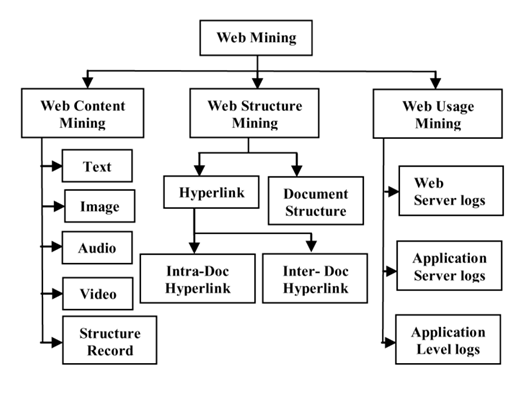
\includegraphics[width = 95mm]{webminingtax}
	\caption{Categorie di Web Mining}
	\label{webminingtax}
\end{figure}

\paragraph{Web Structure Mining}
Il Web Structure Mining � un processo di estrazione di informazioni utili partendo dalla struttura ad hyperlink di un sito Web, che viene considerato come un grafo, i cui nodi sono le pagine e gli archi sono gli hyperlink tra le pagine.
\\
Basata sulla topografia degli hyperlink, il Web Structure Mining pu� categorizzare le pagine web e generare informazioni come la similarit� e le relazioni tra i differenti siti Web \cite{Nilima}.
\\
Tecniche tradizionali di Data Mining non possono generare conoscenza utile perch� non � presente una struttura a link in una tabella relazionale (i.e. database).
\\
Tra i pi� importanti algoritmi che appartengono a questa tipologia si possono trovare Page Rank \cite{pagerankstanford} e HITS \cite{Kleinberg99}, i quali sfruttano la struttura ad hyperlink del Web per assegnare un rank alle pagine, ovvero per restituirle in ordine di importanza relativamente ad una determinata query.

\paragraph{Web Content Mining}
Il Web Content Mining viene usato per cercare informazioni utili dai contenuti delle pagine Web, che possono essere collezioni di testi, immagini, audio, video o dati strutturati incapsulati in liste e tabelle.
\\
Per estrarre il sapere da contenuti pi� complessi, come le immagini, le tecniche di Web Content Mining sono molto limitate \cite{webmining21cap}.
\\
Le tecniche di questa tipologia di Web Mining possono sembrare abbastanza simili alle metodologie tradizionali di Data Mining o di Text Mining, ma le caratteristiche delle pagine Web (e.g. presenza di tag HTML) non permette a queste di essere direttamente applicabili sulle stesse.

\paragraph{Web Usage Mining}
Il Web Usage Mining � l'applicazione delle tecniche di Data Mining per la scoperta di pattern e informazioni utili attraverso l'analisi dei log, che sono immagazzinati nei Web server o nei sistemi che tracciano le attivit� degli utenti.
\\
L'obiettivo di questo campo � la profilazione dell'utente, ovvero analizzare i suoi comportamenti sul web, sia per comprendere quali sono i suoi reali bisogni, sia per offrire dei servizi che possano soddisfare tali necessit� e personalizzare l'esperienza Web.
\\
Questo tipo di Web Mining viene usato in campi disparati, che vanno dalle aziende alle agenzie governative: ad esempio, i siti di e-commerce usano questo tipo di tecnologia per presentare all'utente prodotti per i quali potrebbe essere interessato; le agenzia governative, invece, usano il Web Mining anche per classificare minacce e attentati terroristici.
\\
Alcuni, per�, criticano questa tecnologia: il problema etico di cui pi� si parla � la violazione della privacy, con il rischio di vedere diffusi i propri dati, anche sensibili, senza alcuna consapevolezza da parte dell'utente \cite{612259}.

\section{Rappresentazioni di pagine Web}
\label{webpagerapresentation}
Un sito � formato da pagine Web. Queste sono caratterizzate da numerose rappresentazioni, che sono:

\begin{itemize}
	\item \textbf{Rappresentazione testuale}. Il testo � una componente fondamentale di una pagina Web, poich� ha come scopo il trasferimento dell'informazione. Durante la navigazione, infatti, l'utente estrapola conoscenza semplicemente leggendo il contenuto testuale delle pagine che visita.
	\item \textbf{Rappresentazione visuale}. Quando una pagina Web viene renderizzata da un browser, viene applicato uno stile di formattazione visuale, chiamato CSS, che definisce gli elementi della pagina Web come contenitori rettangolari che sono disposti o uno dopo l'altro o annidati tra loro formando un albero chiamato \texttt{Rendered Box Tree}. L'albero in questione � differente dalla struttura della pagina definita dai tag HTML, poich� una pagina pu� essere ricca di elementi invisibili, come il tag $<$head$>$ o da elementi aventi come stile $display:none$. Inoltre, la generazione del rendered box tree richiede l'esecuzione di codice JavaScript e CSS.
	\item \textbf{Rappresentazione strutturale}. Questa � composta da elementi Web inscritti in tag HTML ed organizzata ad albero. I tag HTML possono essere applicati a porzioni di testo, hyperlink e dati multimediali per fornire loro un significato ed una renderizzazione differente della pagina da parte del browser.
\end{itemize}

In particolare, trattando una pagina Web come un documento testuale, � possibile produrre una rappresentazione vettoriale mediante algoritmi di Word space model, Vector space model, Word embedding (tra cui Word2Vec) per effettuare l'apprendimento. Non solo, trattando tale testo come un paragrafo, � possibile applicare un altro algoritmo di Word embedding, ovvero Doc2Vec.
\\
Ma una pagina Web pu� anche essere trattata come un nodo del sito, il quale non � altro che un grafo, in cui i nodi sono le pagine del sito stesso e gli archi sono gli hyperlink tra i nodi. � possibile, quindi, produrre una rappresentazione vettoriale delle pagine basandosi sulla struttura ad hyperlink del sito. Un esempio � LINE.
\\
Tutti gli algoritmi e le metodologie appena citate verranno descritte nelle sezioni successive.
%L'estrazione di informazione utile, a partire da pagine Web di tipo non strutturato o semi-strutturato � un processo impegnativo.
%\\
%Un modo per affrontare questa sfida � l'applicazione di algoritmi di Machine Learning che possano individuare schemi per estrapolare informazioni utili a partire dai contenuti e dalla struttura delle pagine Web.
%\\
%Per definizione, il Machine Learning � un campo di ricerca, appartenente all'Informatica, che si occupa dello studio della scoperta di pattern. La maggior parte degli algoritmi di Machine Learning trasformano il contenuto di un testo in uno spazio vettoriale \cite{live-2934-4846-jair}, permettendo di estrapolare l'informazione nascosta da testi scritti in linguaggio umano.
%\\
%In questa tesi viene proposto l'utilizzo del modello di spazi vettoriali per rappresentare i vertici del grafo della pagina Web. Per spiegare che cos'� e perch� � importante il modello di spazio vettoriale, occorre specificare e descrivere l'argomento di quello dello spazio delle parole (Word space model), che sono strettamente collegati l'uno all'altro.

\subsection{Word space model}
Il Word Space Model, come definito in \cite{wordspacemodel}, � una rappresentazione spaziale del significato delle parole. Si basa sul fatto che la similarit� semantica viene rappresentata come prossimit�, in uno spazio ad $n$ dimensioni, dove $n$ � un intero.

\begin{figure}[h]
	\centering
	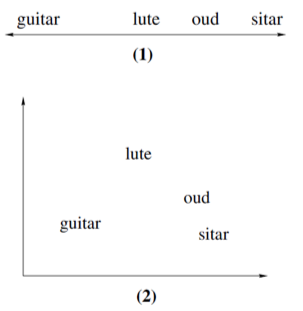
\includegraphics[width = 50mm]{wordspaceexample}
	\caption{Esempi di spazi di parole, rispettivamente mono-dimensionale (1) e bi-dimensionale (2)}
	\label{wordspaceexamples}
\end{figure}

In Figura \ref{wordspaceexamples} sono riportati due esempi di spazi di parole, in cui la prossimit� � data dalla posizione delle parole nello spazio.
In entrambi i casi, si pu� notare come il termine $sitar$ sia pi� simile di significato a $oud$, e meno simile a $guitar$.
\\
Ma come si costruisce uno spazio delle parole? Una modalit� di costruzione � la \textbf{matrice di co-occorrenze}. Tale matrice pu� essere formata sia parola per parola ($w$ x $w$), dove $w$ sono i tipi di parole nel set, sia parola per documento ($w$ x $d$), dove $d$ sono i documenti nel set. Le celle di questa matrice registrano la frequenza di occorrenza della parola i-esima in un contesto j-esimo, oppure in un documento j-esimo nel caso di matrice parola per documento.
\\\\
Per spiegare la matrice di co-occorrenze prendiamo come esempio la frase:
\begin{figure}[h]
	\centering
	Whereof one cannot speak thereof one must be silent
	\label{sentencematrix}
	\caption{Frase di esempio per la matrice di co-occorrenze \cite{wordspacemodel}}
\end{figure}

\begin{table}[h]
	\centering
	\caption{Matrice di co-occorrenze parola per parola \cite{wordspacemodel}}
	\label{tablematrix}
	\begin{tabular}{|l|l|l|l|l|l|l|l|l|}
		\hline
		& whereof & one & cannot & speak & thereof & must & be & silent  \\ \hline
		whereof & 0 & 1 & 0 & 0 & 0 & 0 & 0 & 0  \\ \hline
		one & 1 & 0 & 1 & 0 & 1 & 1 & 0 & 0 \\ \hline
		cannot & 0 & 1 & 0 & 1 & 0 & 0 & 0 & 0 \\ \hline
		speak & 0 & 0 & 1 & 0 & 1 & 0 & 0 & 0 \\ \hline
		thereof & 0 & 1 & 0 & 1 & 0 & 1 & 0 & 0 \\ \hline
		must & 0 & 1 & 0 & 0 & 1 & 0 & 1 & 0 \\ \hline
		be & 0 & 0 & 0 & 0 & 0 & 1 & 0 & 1 \\ \hline
		silent & 0 & 0 & 0 & 0 & 0 & 0 & 1 & 0 \\ \hline
	\end{tabular}
\end{table}

Le celle della matrice di co-occorrenze, visibile nella Tabella \ref{tablematrix}, registrano le occorrenze delle parola i-esima, le quali dipendono dal contesto. Con il termine \textit{contesto} si intende un insieme di parole che si trovano nelle vicinanze della parola i-esima.
\\
Queste liste di occorrenze sono dei veri e propri vettori. Un vettore, per definizione, � un elemento di uno spazio vettoriale, ed � definito da $n$ componenti o coordinate $\overrightarrow{v} = (x_1, x_2, ..., x_n)$ \cite{wordspacemodel}. Tali coordinate definiscono la posizione nello spazio n-dimensionale.
\\
Quindi, la matrice di co-occorrenze non � altro che una realizzazione del modello dello spazio vettoriale, chiamato Vector Space Model.

\paragraph{Vector Space Model}
\label{tfidf}
Il Vector Space Model � una modalit� algebrica per rappresentare documenti di testo come vettori, inseriti in uno spazio vettoriale.
\\
Generalmente, per definire i vettori viene usato come peso \textit{tf-idf}, una funzione che viene usata per misurare l'importanza di un termine rispetto ad un documento o ad una collezione di documenti. Come suggerisce il nome, � composta da due fattori: \textit{tf} e \textit{idf}.
\\
\textit{Tf}, abbreviazione di \textit{term frequency}, misura quante volte un termine appare in un documento. Dato che ogni documento ha lunghezza differente, ovvero � composto da un differente numero di parole, � possibile che un termine possa apparire molte pi� volte nei documenti pi� lunghi rispetto a quelli pi� corti. Questo problema viene risolto dividendo la frequenza dei termini per la lunghezza del documento. La formula �:
\begin{equation}
	tf_{i, j} = \frac{n_{i, j}}{|d_J|}
\end{equation}
dove $n_{i, j}$ � il numero di occorrenze del termine $t_i$ che si trova nel documento $d_j$, mentre il denominatore � la dimensione del documento $d_j$.
\\
\textit{Idf}, abbreviazione di \textit{inverse document frequency}, misura invece i termini che si presentano pi� volte in un documento, ma con meno frequenza in tutta la collezione di documenti. Questo perch� potrebbero esserci dei termini  pi� significativi che appaiono raramente in un determinato elaborato, ma frequentemente nel set di documenti. La formula �:
\begin{equation}
	idf_i = \log{\frac{|D|}{|\{d : t_i \in d\}|}}
\end{equation}
dove $|D|$ � il numero di documenti presenti nella collezione, mentre il denominatore � il numero di documenti che contengono il termine $t_i$.
\\\\
Il modello di spazio vettoriale sopra descritto, per�, presenta particolari problematiche quando si vuole costruire uno spazio delle parole: da un lato, se non si hanno sufficienti dati, non sar� possibile costruire, in maniera fedele, un modello di distribuzione delle parole; dall'altro, se tale spazio vettoriale sar� dimensionalmente grande, innalzer� la complessit� computazionale.
\\
Secondo la sperimentazione portata avanti da \cite{wordspacemodel}, � stato riscontrato un altro problema: nella matrice di co-occorrenze circa il 99\% delle celle conterr� zero come valore. Solo una parte delle parole apparir� realmente. Questo fenomeno � un esempio dell'applicazione della \textit{Zipf's law}, una legge empirica che deriva dalla frequenza di un evento $P_i$, che fa parte di un insieme, in funzione della posizione $i$ chiamata \textit{rango} nell'ordimanto decrescente rispetto alla frequenza stessa di tale evento. La formula della legge � la seguente:
\begin{equation}
	f(P_i) = \frac{c}{i}
\end{equation}
dove $i$ indica il rango, $P_i$ indica l'evento che occupa l'i-esimo rango (ovvero l'i-esimo evento pi� frequente), $f(P_i)$ � il numero di volte (frequenza) che si verifica l'evento $P_i$, c � una costante di normalizzazione, pari al valore $f(P_i)$.
\\\\
Una possibile soluzione alle situazioni problematiche sopra descritte � la riduzione della dimensione (\textit{dimensional reduction}): un processo di compressione di uno spazio multi dimensionale ad uno avente bassa dimensione, causando anche la riduzione della grandezza della matrice e del numero di zero ivi inseriti.
\\
Una tecnica di riduzione della dimensione pi� utilizzata � \textit{t-SNE}, che � particolarmente adatta per comprimere uno spazio vettoriale di grandi dimensioni in uno avente uno, due o tre dimensioni, per poi essere visualizzato in un grafico di dispersione. Questo tipo di grafico � un sistema gli assi cartesiani di uno, due o tre dimensioni. Una volta effettuata la riduzione, i valori ottenuti per ciascun elemento del set vengono usati per posizionarlo nello spazio.

\begin{figure}[h]
	\centering
	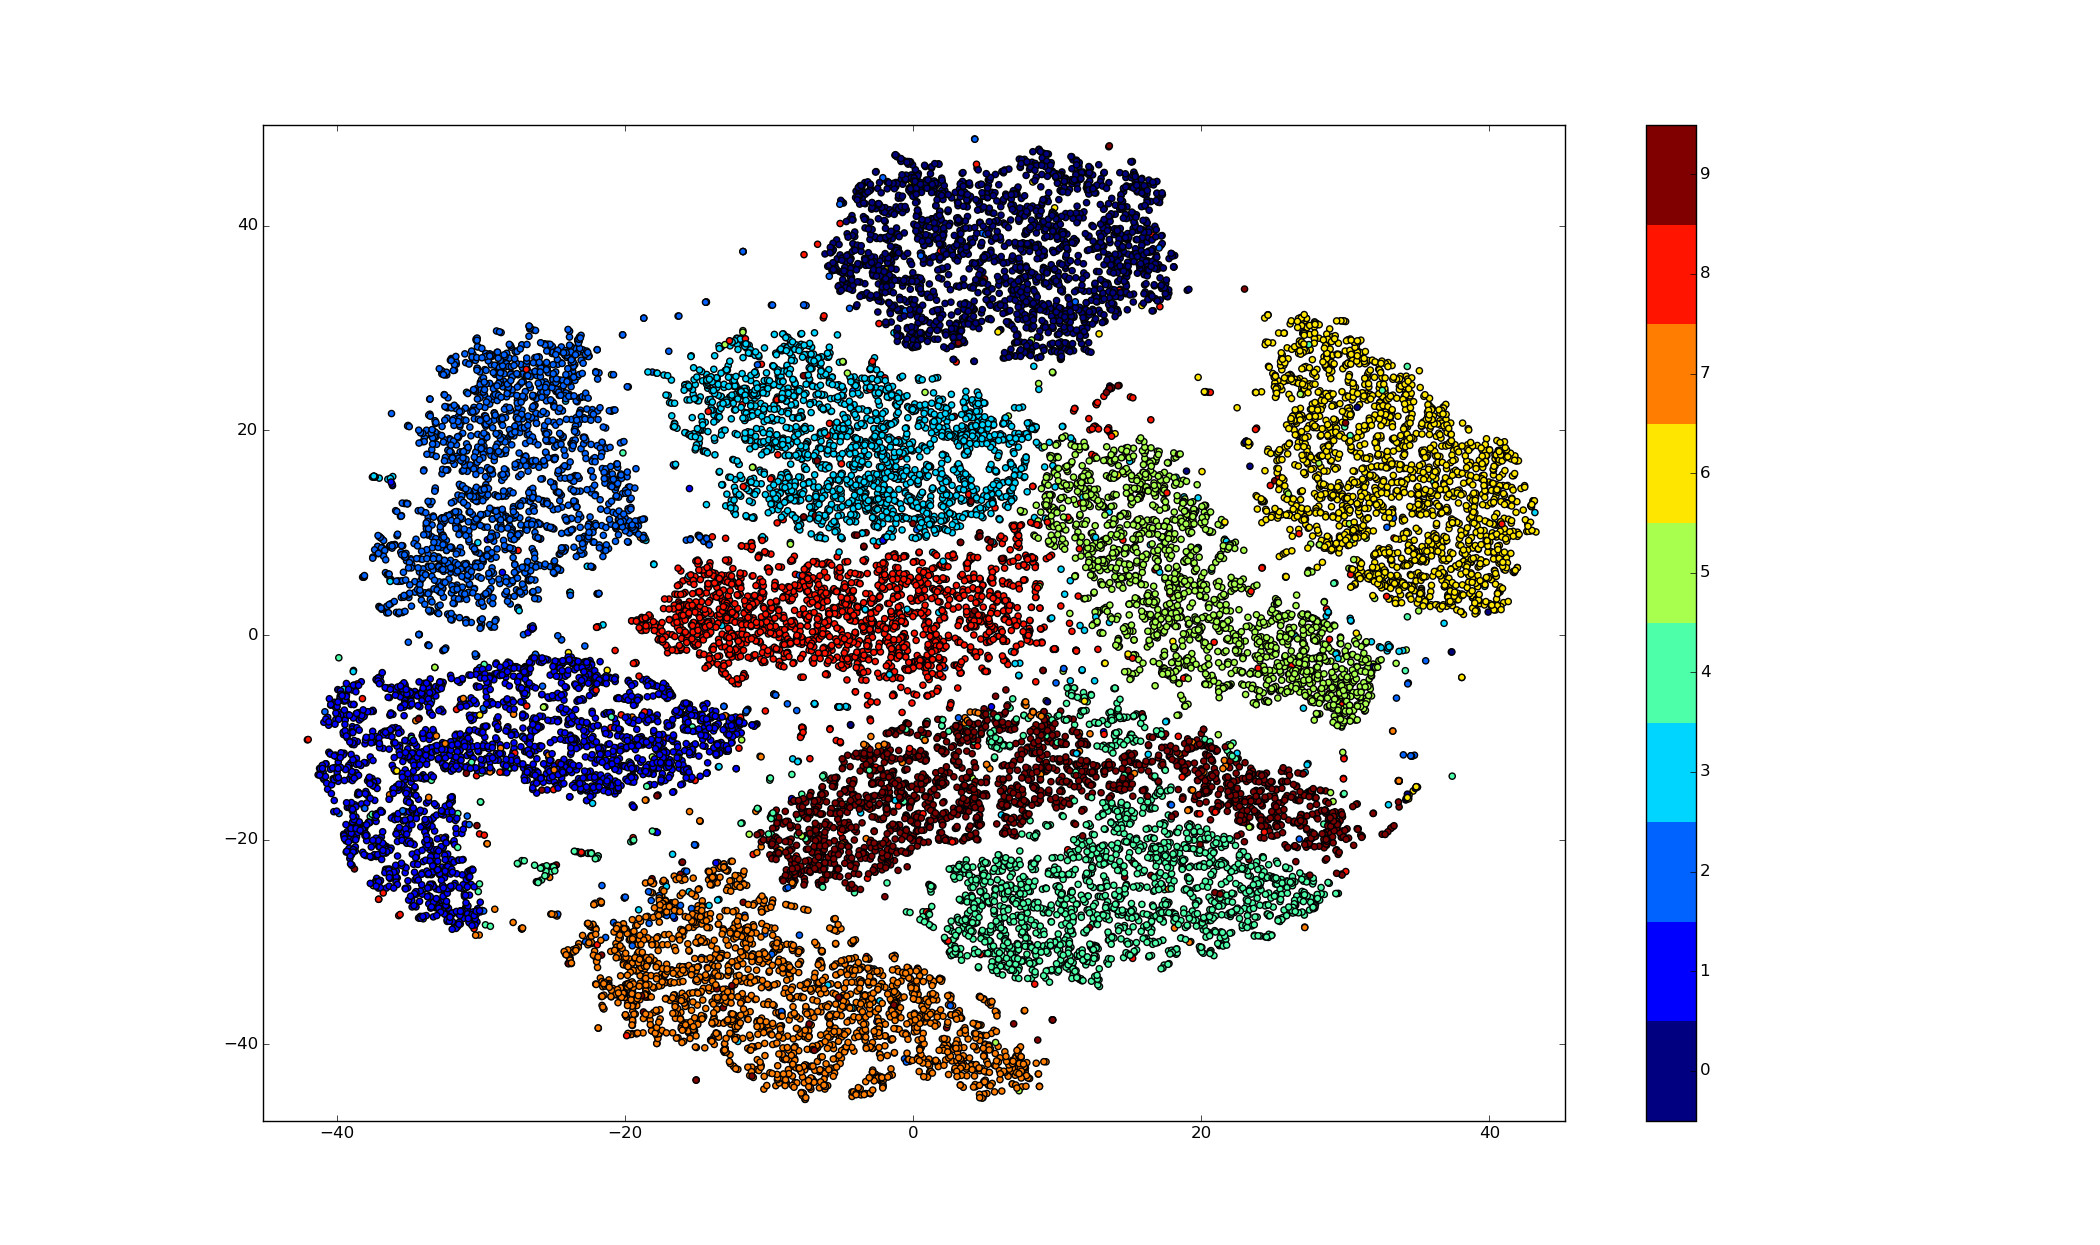
\includegraphics[width = 160mm]{tsne}
	\caption{Esempio di grafico di dispersione}
	\label{tsne}
\end{figure}

\paragraph{Word embedding}
La funzione peso \textit{tf-idf} non � la sola usata per costruire uno spazio dei vettori: nelle tecniche di Data Mining, che sfruttano gli algoritmi di Machine Learning, ci si sta orientando sempre pi� sull'uso delle reti neurali per estrarre conoscenza partendo da una collezione di dati.
\\
Questo � il Word Embedding, nome di una serie di tecniche per il language modeling e per il Feature Learning nel campo del Natural Language Processing \cite{bengio03}, in cui ad ogni parola viene associato un vettore chiamato \textit{Feature Vector}.
\\
Il Word Embedding � una funzione parametrizzata
\begin{equation}
	W : words \to \mathbb{R^n}
\end{equation}
che trasforma le parole di un dato linguaggio in un vettore multidimensionale. Per esempio:
\begin{equation}
	W("mat") = (0.0, 0.6, -0.1, ...)
\end{equation}
Partendo da un documento, � possibile trasformare i termini in vettori, formando un vero e proprio spazio vettoriale, chiamato anche Word Embeddings Space.

\begin{figure}[h]
	\centering
	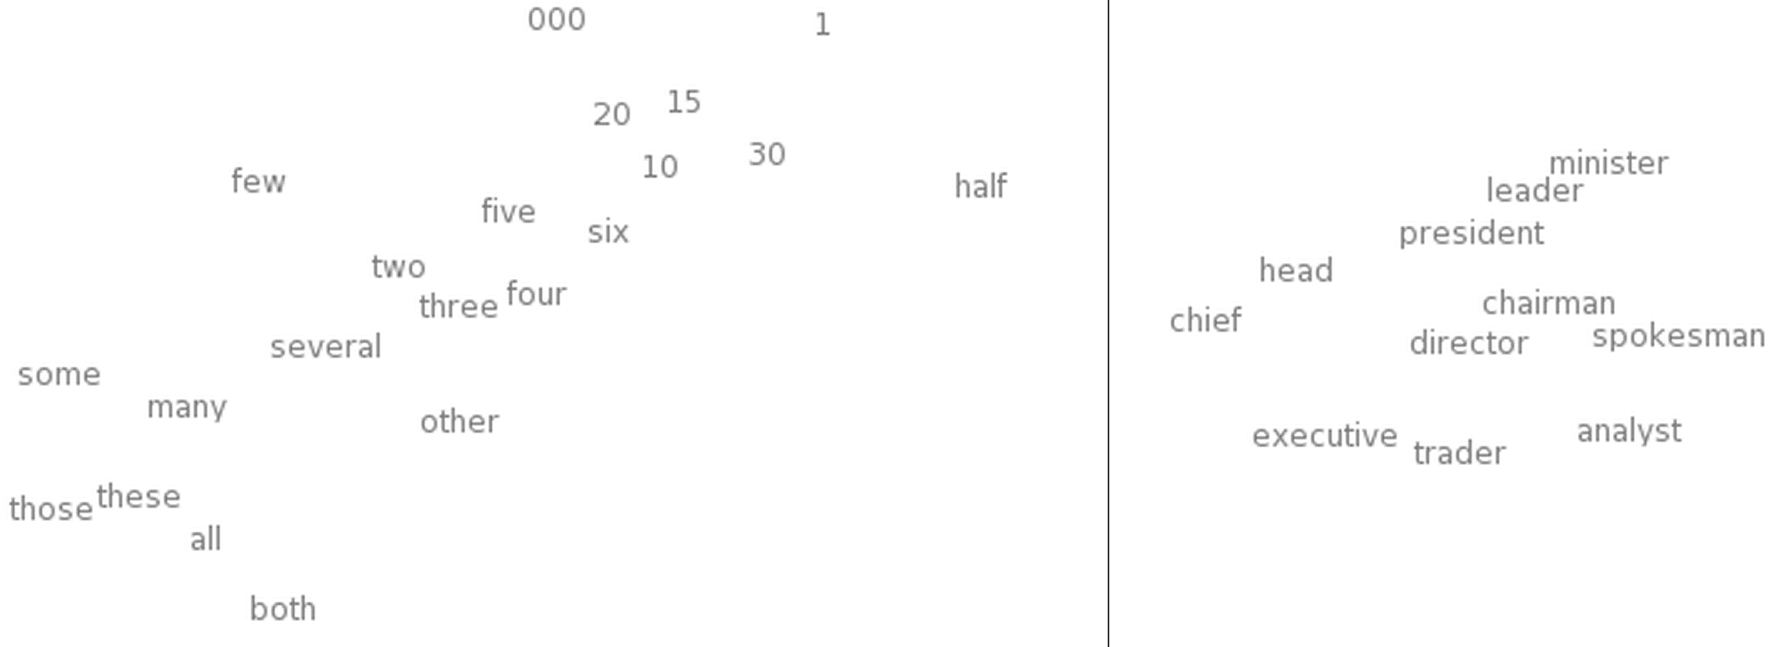
\includegraphics[width = 150mm]{tsneplot}
	\caption{Esempio di spazio degli embeddings}
	\label{tsneplot}
\end{figure}

In Figura \ref{tsneplot} � possibile notare come parole simili si trovano vicine tra loro: la parola \textit{three} � molto vicina alle parole \textit{two} e \textit{four}. Questo � dovuto al fatto che tali parole hanno vettori simili. Infatti, se si usa un sinonimo, la validit� della frase non cambia (per esempio: "poche persone cantano bene" $\to$ "un paio di persone cantano bene"), perch� le parole "poche" e "paio" sono vicine tra loro ed hanno vettori simili.
\\\\
Un'altra propriet� interessante della funzione di Word Embedding � l'analogia tra le parole, nascosta nella differenza dei loro vettori:
\begin{equation}
	W("woman") - W("man") \simeq W("queen") - W("king")
\end{equation}
Da questo si evince che c'� una correlazione tra parole che hanno genere opposto, in quanto appariranno in contesti simili, differenti solo per alcuni dettagli come pronomi o articoli. Lo stesso principio vale per parole singolari e plurali \cite{mikolov13}.
\\\\
Apprendere dei termini e trasformarli in Feature Vectors rappresenta una base per effettuare operazioni di Data Mining, come per esempio il raggruppamento dei termini appresi in gruppi attraverso il Clustering, usando qualche funzione di similarit�. Si approfondiranno tali funzioni nella Sezione \ref{distancefunctions}.

\subsection{Word2Vec}
\label{word2vec}
Word2Vec � un algoritmo di Word Embedding ed � una rete neurale a due livelli che apprende le parole da un testo in input, le quali vengono trasformate in vettori chiamati Feature Vectors. Viene considerato erroneamente come un deep-learning (apprendimento approfondito): in realt� si tratta di un apprendimento di tipo superficiale (shallow-learning).
\\\\
L'output di questa rete neurale � un vocabolario in cui ogni termine ha un vettore, che pu� essere compreso da una rete di deep-learning o semplicemente interrogato per rilevare delle relazioni tra i termini.

\begin{figure}[h]
	\centering
	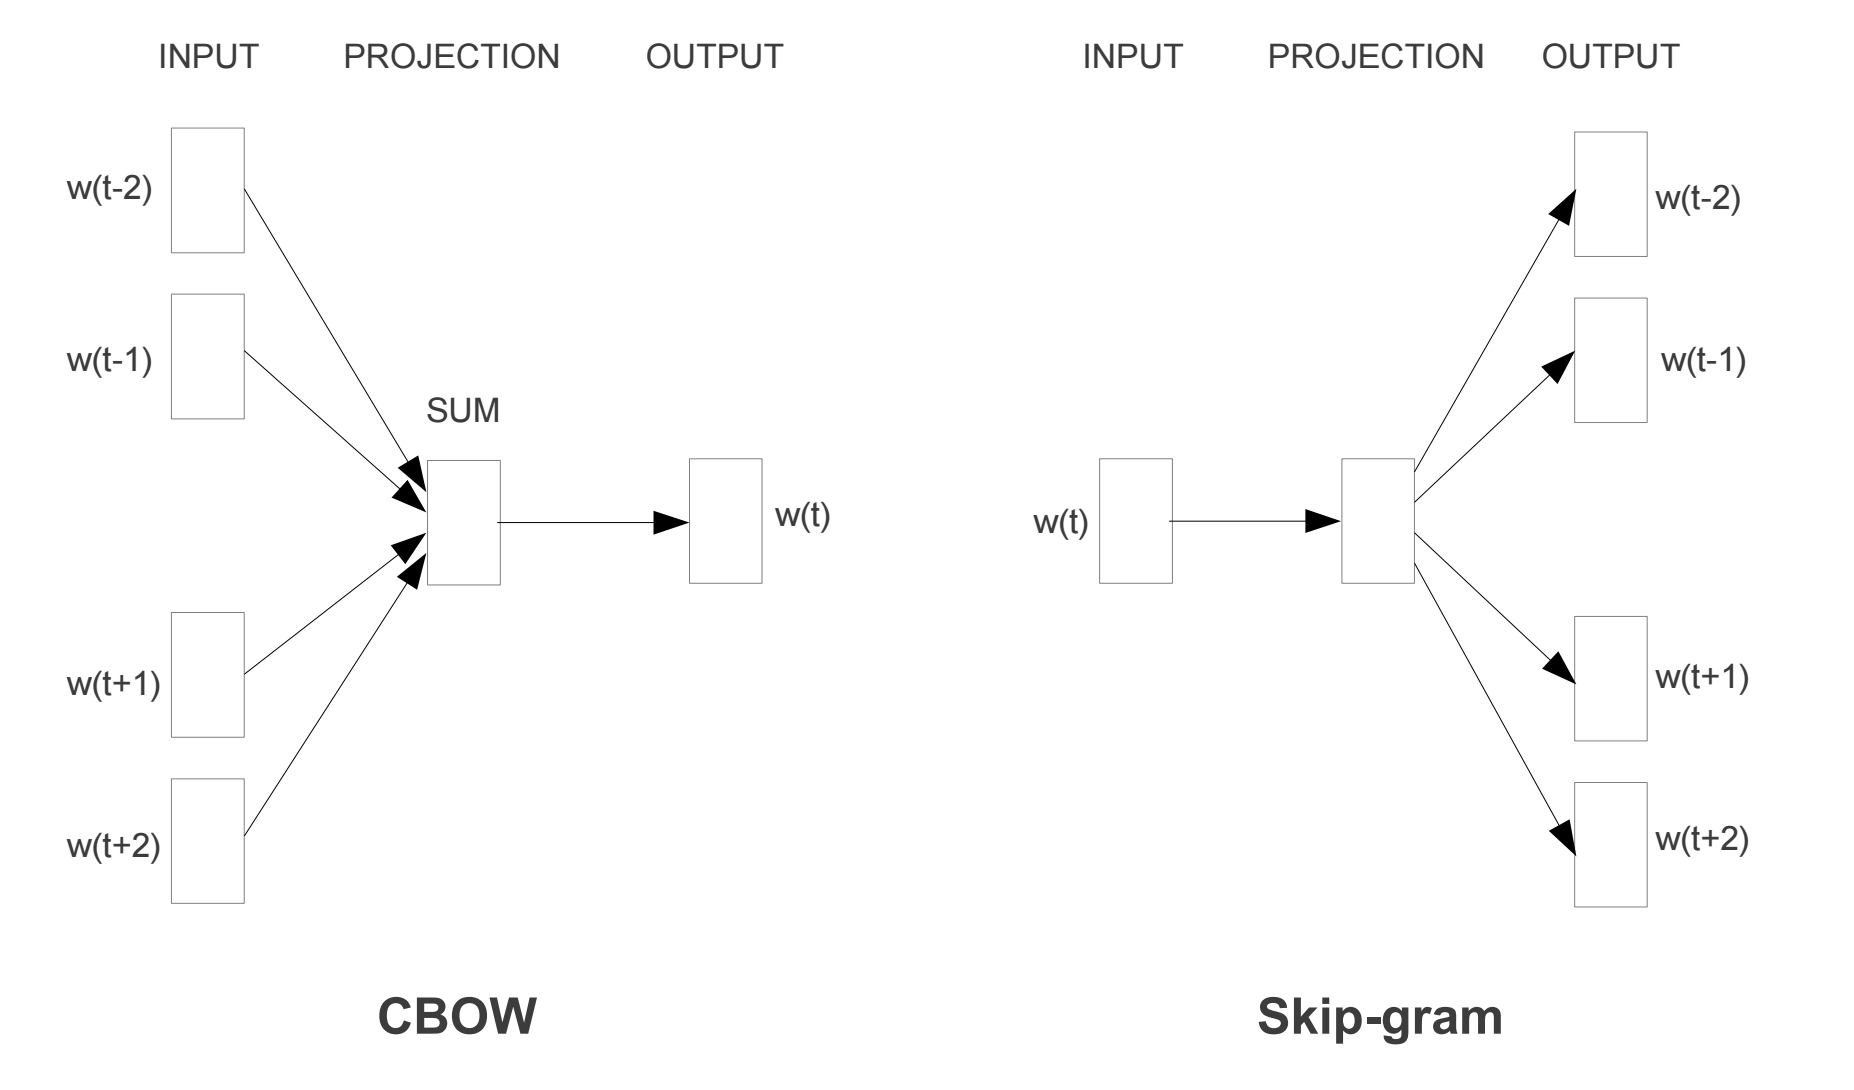
\includegraphics[width = 150mm]{word2vecmodels}
	\caption{I modelli di apprendimento di Word2Vec}
	\label{word2vecmodels}
\end{figure}

Word2Vec � composto da due modelli di apprendimento: \textbf{CBOW} (continuous bag of words) e \textbf{Skip-Gram}.
\\\\
\textbf{CBOW} consiste nel predire una determinata parola a partire dal suo contesto, che � composto dal numero di parole che vengono prese in considerazione durante l'apprendimento. Questo modello di apprendimento tratta l'intero contesto come una sola osservazione. Generalmente, CBOW restituisce risultati pi� accurati con piccole collezioni di dati \cite{mikolov}.
\\\\
\textbf{Skip-Gram}, invece, � l'inverso di CBOW: predice il contesto a partire da una parola.\\
Questo modello di apprendimento tratta ogni coppia contesto-obiettivo come una nuova osservazione, rendendo i risultati pi� accurati quando si hanno grandi collezioni di dati \cite{mikolov}.
\\
L'obiettivo dell'apprendimento di questo modello � quello di trovare le rappresentazioni vettoriali delle parole utili per predire quelle circostanti in una frase o in un documento. Formalmente, data una sequenza di parole $w_1, w_2, ..., w_T$ viene costruito un vocabolario, i cui termini hanno un vettore con $n$ dimensione generato casualmente. Skip-Gram deve massimizzare la probabilit� media logaritmica:
\begin{equation}
\label{skipgrameq}
	\frac{1}{T} \sum_{t=1}^{T} \sum_{-c \le j \le c, j \neq 0} \log p(w_{t+j}|w_t)
\end{equation}
dove $c$ � la dimensione della finestra di contesto, $w_t$ � la parola in input e $w_{t+j}$ � la parola in analisi del contesto.
\\
Per capire meglio questo tipo di modello di apprendimento, analizziamo questa frase:
\begin{figure}[h]
	\centering
	The quick brown fox jumped over the lazy dog.
\end{figure}
\\
Inizialmente, si crea il set di dati formato da coppie (contesto, parola), di cui il primo � una sequenza di parole che dipende dalla dimensione della finestra, mentre la parola � il termine che si sta esaminando. Quindi, se si ha una finestra di contesto di dimensione 1, il set di dati sar�:

\begin{figure}[h]
	\centering
	([quick], the), ([the, brown], quick), ([quick, fox], brown), [...] $\to$ (the, quick), (quick, the), (quick, brown), (brown, quick), [...]
\end{figure}

Supponiamo di trovarci al passo $t$, dove si trova il primo caso di apprendimento (the, quick). L'obiettivo � quello di predire \textit{quick} da \textit{the}, applicando la formula \ref{skipgrameq} e massimizzando la probabilit� media logaritmica per apprendere il vettore ottimale di \textit{quick}. Cos� facendo le parole simili avranno vettori simili. Ad ogni passo vengono aggiornati i vettori delle parole precedentemente apprese. Questo processo di apprendimento viene ripetuto sull'intera collezione di dati.

\subsection{Doc2Vec}
\label{doc2vec}
Doc2Vec, chiamato anche Paragraph2Vec, � un'estensione di Word2Vec che apprende correlando etichette e parole, invece che parole con altre parole.
\\
Differentemente da Word2Vec, che converte una parola in un vettore, Doc2Vec aggrega tutte le parole di un paragrafo in un vettore.
\\
Quindi, data una collezione di testi che possa essere divisa in $n$ documenti, o paragrafi, ad ogni paragrafo � assegnato un vettore. Il processo di apprendimento � caratterizzato dallo spostamento della finestra delle parole di contesto attraverso ogni parola di ogni paragrafo, per ogni paragrafo \cite{HongSeokho}.
\\
L'idea di base � quella di apprendere vettori di paragrafi in maniera simile all'apprendimento dei vettori delle parole. Vengono create due matrici: una formata dai vettori dei paragrafi appresi e l'altra da quelli delle parole. Il vettore del paragrafo � condiviso per tutte le parole che si trovano nello stesso, ma non per gli altri paragrafi. Gli embedding dei vettori e dei paragrafi sono combinati durante l'apprendimento ed aggiornati mediante la concatenazione o la media. I vettori vengono appresi utilizzando coppie, composte dalla parola da predire e dal contesto del campione, contrassegnato da un identificativo del paragrafo \cite{mirela}.
%\\
%Come Word2Vec, Paragraph2Vec ha due modelli di apprendimento:
%\begin{itemize}
%	\item \textbf{Distributed Memory}. Simile al modello CBOW di Word2Vec. Dati in input $N$ paragrafi e $M$ parole, viene casualmente inizializzata una matrice di embedding $D$ per i paragrafi ed una $W$ per le parole. Per ogni paragrafo si predice la successiva parola effettuando la media o il concatenamento dei vettori di paragrafo e dei termini nella finestra di contesto, che scorre per tutta la lunghezza del paragrafo stesso, non modificando il suo vettore. Una volta che viene completato il paragrafo, vengono aggiornate le matrici $D$ e $W$.
%	\item \textbf{Distributed Bag of Words}. Simile al modello Skip-Gram di Word2Vec. Vengono predette le parole che si trovano in un paragrafo dando solo il suo vettore. Questo modello � concettualmente pi� semplice e pi� efficiente in termini di memoria.
%\end{itemize}

\subsection{LINE}
\label{line}
LINE � un nuovo modello di apprendimento, capace di produrre rappresentazioni vettoriali (embedding) di vertici in una rete o grafo. Un grafo � una coppia ordinata $G = (V, E)$ di insiemi, con $V$ insieme dei nodi ed $E$ insieme degli archi.
\\
Questo modello di apprendimento lavora bene soprattutto con grafi orientati, pesati e non-pesati. Viene richiesto come input un file contenente gli archi che costituiscono il grafo da apprendere. L'obiettivo � quello di rappresentare ogni vertice $v \in V$ in un vettore $R^d$ applicando una funzione $f_G : V \to R^d$, dove $d << |V|$ \cite{tang2015line}. Viene prodotto, infine, uno spazio vettoriale formato da rappresentazioni vettoriali dei singoli nodi del grafo appreso.% Ogni vettore $R^d$ preserva la prossimit� di primo e secondo ordine tra i vertici.
\\
LINE preserva sia la prossimit� di primo che di secondo ordine. Nel primo caso ottimizza la seguente funzione di perdita:
\begin{equation}
\label{firstorderprox}
	- \sum_{(i,j) \in E} w_{ij} \log p_1(v_i, v_j)
\end{equation}
Trovando un insieme $\{\vec{u}_i\}_{i=1...|V|}$ che minimizza la funzione obiettivo \ref{firstorderprox}, � possibile rappresentare ogni vertice in uno spazio $d$-dimensionale. Anche nel secondo caso, si cerca di ottimizzare la seguente funzione di perdita:
\begin{equation}
\label{secondorderprox}
	- \sum_{(i,j) \in E} w_{ij} \log p_2(v_j|v_i)
\end{equation}
Trovando due insiemi $\{\vec{u}_i\}_{i=1...|V|}$ e $\{\vec{u}^{'}_i\}_{i=1...|V|}$ che minimizzano la funzione obiettivo \ref{secondorderprox}, � possibile rappresentare ogni vertice $v_i$ con un vettore $d$-dimensionale $\vec{u}_i$.

\begin{figure}[h]
	\centering
	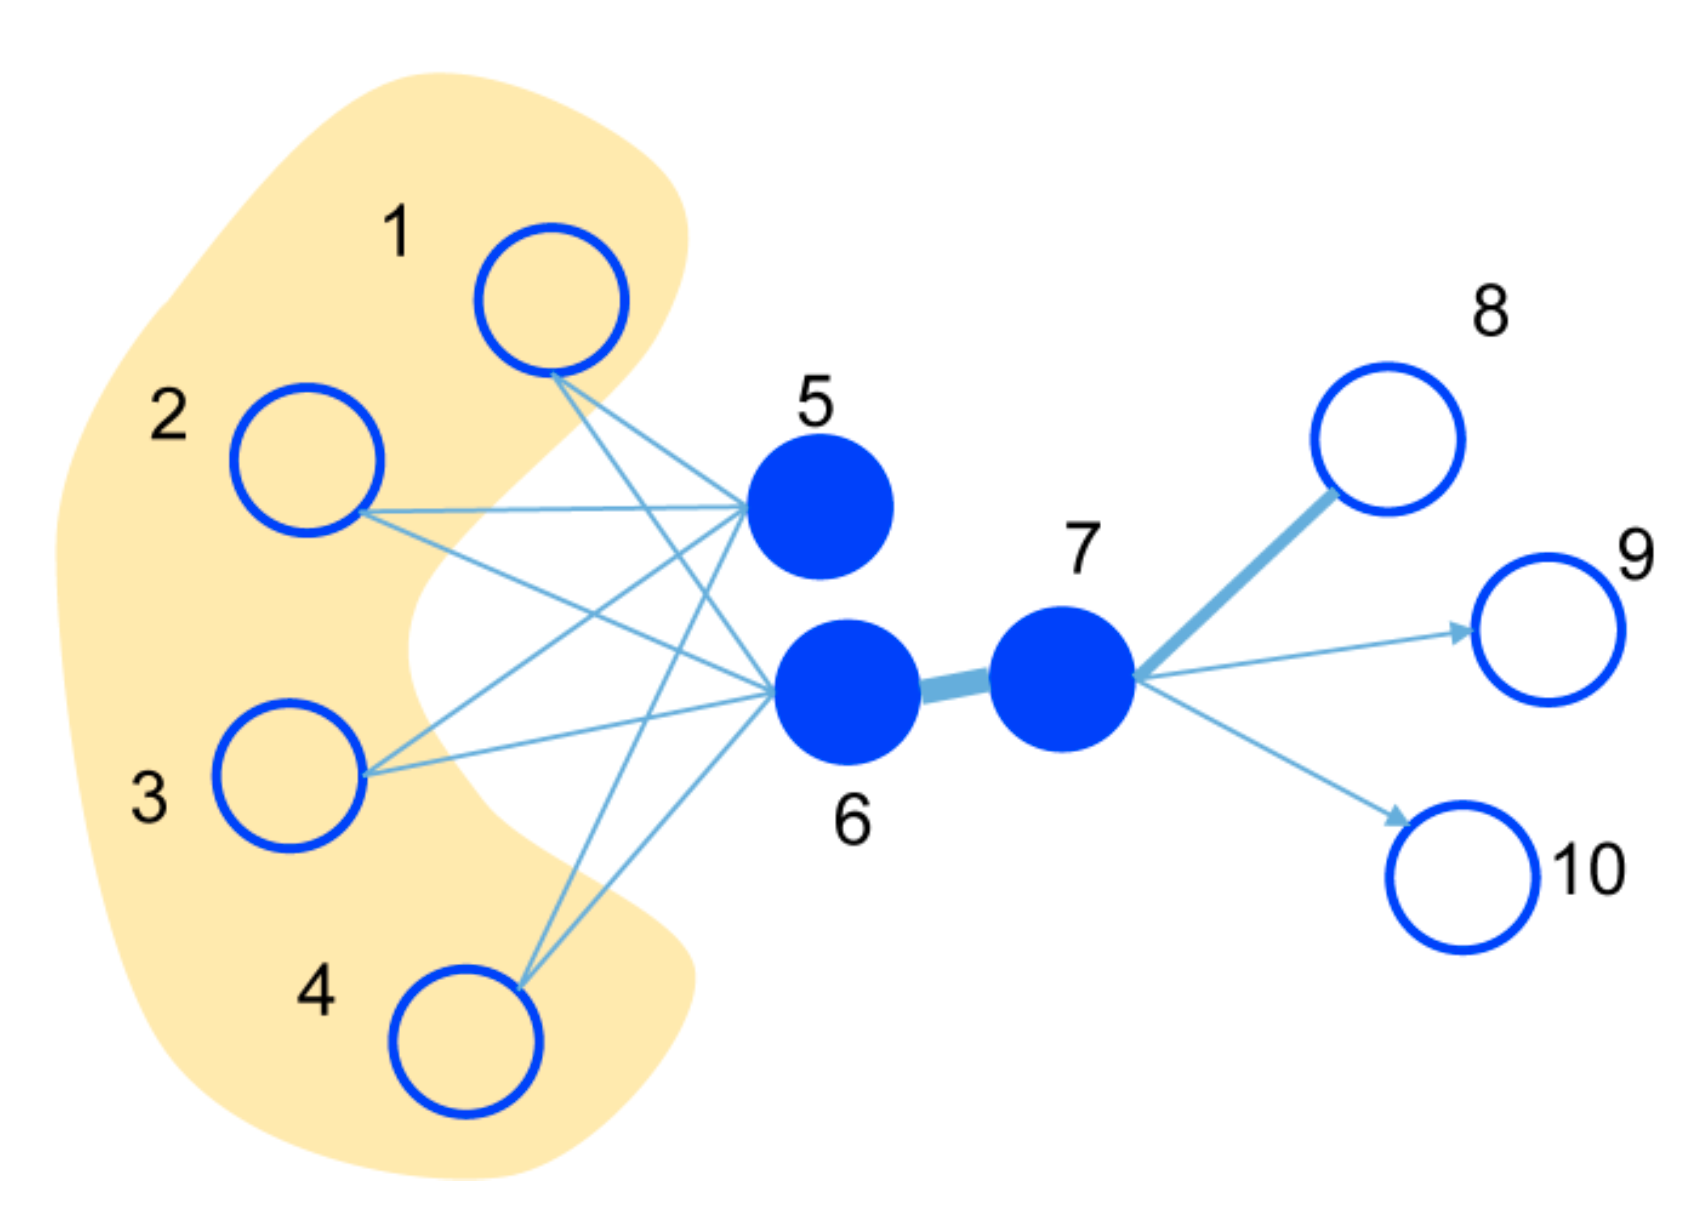
\includegraphics[width = 100mm]{infonet}
	\caption{Un esempio di grafo/network di informazioni \cite{tang2015line}}
	\label{infonet}
\end{figure}

Per spiegare la prossimit� di primo e secondo ordine, analizziamo la Figura \ref{infonet}. I vertici 6 e 7 sono collegati da un arco avente un determinato peso: tale peso indica la prossimit� di prim'ordine. Nel caso dei vertici 6 e 8, dato che non esiste un arco tra questi due, la prossimit� di primo ordine � 0.
\\
I vertici 5 e 6, invece, condividono molti vertici vicini: hanno un'alta prossimit� di secondo ordine.
\\
In altre parole, la prossimit� di primo ordine implica la somiglianza di due nodi. Per esempio, persone che sono amici gli uni con gli altri in un social network tendono a condividere simili interessi; pagine che sono collegate le une alle altre nel World Wide Web tendono a riferirsi a simili argomenti. La tipologia di secondo ordine, invece, sono persone, in un social network, che condividono simili amici che tendono ad avere simili interessi; parole che co-occorrono sempre con lo stesso insieme di termini tendono ad avere significati simili.
\\
Pu� capitare che una coppia di nodi di un grafo possa non avere un arco, avendo come prossimit� di primo ordine 0, anche essendo simili. Per questo la prossimit� di primo ordine non � sufficiente per preservare le strutture del network, ed � importante considerare una nozione alternativa di prossimit� che permetta di considerare i vertici come simili, se condividono simili nodi vicini (prossimit� di secondo ordine). LINE, quindi, permette di apprendere sia le strutture locali (i.e. i diretti vicini) sia quelli globali (i.e. i vicini dei vicini) del network.
\\
La situazione sopra descritta � riscontrabile anche in Word2Vec. Analizzare solo le parole immediatamente vicine al termine target non permette di considerare quelle simili che non si trovano vicine le une alle altre. Per questo � possibile modificare la dimensione della finestra di contesto per apprendere parole che non si trovano nell'immediato vicinato del termine target.
\\
Rispetto a LINE, che permette al pi� di analizzare i vicini dei vicini di un dato vertice (quindi relazioni avente profondit� 2), Word2Vec permette di analizzare relazioni pi� ampie, aventi profondit� maggiori di 2.
%Se due vertici hanno un'alta prossimit� dovrebbero essere rappresentati nello spazio degli embeddings vicini tra loro. Ancora, in \cite{tang2015line} si � osservato come la prossimit� di primo ordine, nel mondo reale, non � sufficiente per preservare le strutture del network globali. Per questo motivo, nella sperimentazione effettuata in \cite{tang2015line}, � stata esplorata la prossimit� di secondo ordine.
%\\
%Tali prossimit�, tuttavia, sono complementari l'una all'altra.

\section{Clustering}
\label{Clustering}
Le classi, insiemi di oggetti che condividono determinate caratteristiche, hanno un ruolo importante sia nell'analisi effettuata da persone, sia nella descrizione del mondo. Infatti, gli esseri umani hanno l'abilit� di dividere gli oggetti in gruppi e di assegnarli a questi insiemi \cite{ch8}. 
\\
Questo processo di divisione prende il nome di Clustering ed ha come scopo quello di selezionare e raggruppare, da una collezione di dati, elementi omogenei, avendo come base la somiglianza tra gli stessi.
\\
L'attivit� di raggruppamento pu� essere applicata in molti campi \cite{ch8}:
\begin{itemize}
	\item \textbf{Biologia}. Tecniche di Clustering sono state applicate per analizzare informazioni genetiche e creare una tassionomia di tutte le specie viventi.%La ricerca scientifica ha investito molto tempo per creare una tassionomia di tutte le specie viventi, basandosi sul regno, classe, ordine, famiglia, geni e specie. Non solo, tecniche di Clustering sono state applicate per analizzare una grande quantit� di informazioni genetiche: sono stati raggruppati geni che hanno funzioni simili.
	\item \textbf{Clima}. Il Clustering � stato utilizzato per trovare degli schemi nel clima della Terra.%Per capire il clima della Terra bisogna trovare degli schemi nell'atmosfera e negli oceani. Il Clustering � stato applicato per scoprirli, analizzando la pressione atmosferica delle regioni polari e nelle aree di oceano che hanno un impatto significativo sul clima della terra ferma.
	\item \textbf{Psicologia e Medicina}. Le operazioni di Clustering hanno identificato variazioni di malattie e depressioni.%Una malattia ha un incredibile numero di variazioni, e le operazioni di Clustering possono essere usate per identificare queste sottocategorie. Per esempio, � possibile applicare questo processo per scoprire tipologie differenti di depressione.
	\item \textbf{Business}. Il Clustering viene usato per dividere i consumatori in gruppi per successive attivit� di analisi e di marketing.%Il campo del Business raccoglie una quantit� enorme di informazioni di clienti potenziali ed effettivi. Il Clustering pu� essere usato per dividere i consumatori in gruppi per successive attivit� di analisi e di marketing.
	\item \textbf{Information Retrieval}. Il World Wide Web � un enorme contenitore di pagine Web, ed una semplice ricerca pu� dare come risultato milioni di pagine. Le tecniche di Clustering vengono usare per dividerle in gruppi, ognuno dei quali cattura un aspetto particolare dell'interrogazione. Quindi, se si cerca, con un motore di ricerca, la parola \textit{film}, verranno restituite pagine Web raggruppate in categorie come recensioni, trailer, celebrit�, teatri e cinema. Ogni categoria (cluster) pu� essere diviso in sottogruppi (sottocluster) e si produrr� una struttura gerarchica che servir� all'utente per effettuare altre ricerche.
\end{itemize}

%\subsection{Approcci di Clustering}
Quindi, l'operazione di Clustering � essenzialmente la creazione di un insieme di Cluster (i.e. un insieme di insiemi), che generalmente contengono tutti gli elementi iniziali.
\\
In questa tesi sono stati utilizzati algoritmi di Clustering che si basano sulla rappresentazione vettoriale degli elementi (i.e. pagine di un sito Web) per poter raggrupparli in insiemi.
\\
Esistono vari approcci di Clustering per raggruppare elementi in insiemi. Alcuni di questi sono:
\begin{itemize}
    \item Hard Clustering o Soft Clustering
    \item Partizionali o gerarchici
\end{itemize}

\paragraph{Hard Clustering e Soft Clustering}
Questi algoritmi attuano un approccio secondo cui un elemento pu� essere assegnato ad un solo Cluster o a pi� Cluster. Con Hard Clustering intendiamo che l'algoritmo assegna un elemento ad uno ed un solo Cluster; con Soft Clustering, invece, l'elemento pu� essere assegnato a pi� Cluster con gradi di appartenenza diversi.

\paragraph{Clustering partizionale}
Gli algoritmi di Clustering partizionali creano una divisione delle osservazioni minimizzando una certa funzione di costo:
\begin{equation}
   {\textstyle \sum_{j=1}^{k}} E(C_j)
\end{equation}
dove $k$ � il numero desiderato di Cluster, $C_j$ � il j-esimo Cluster ed $E : C \to \mathbb{R^+}$ � la funzione di costo associata al singolo Cluster. L'algoritmo pi� famoso che fa parte di questa categoria � K-Means.

\paragraph{Clustering gerarchico}
Gli algoritmi che fanno parte di questa categoria non suddividono lo spazio, bens� costruiscono una gerarchia di Cluster. In questa strategia rientrano due sottotipi:
\begin{itemize}
\item \textbf{Aggregativo}: tale approccio considera $n$ Cluster per $n$ elementi, cio� ogni elemento viene considerato un Cluster a s�. Successivamente, l'algoritmo unisce tutti i Cluster pi� vicini. Viene anche chiamato bottom-up.
\item \textbf{Divisivo}: tale approccio opera in maniera opposta rispetto al precedente, poich� tutti gli elementi vengono considerati come un unico Cluster e l'algoritmo deve dividere il Cluster in insiemi aventi dimensioni inferiori. Questa metodologia viene anche chiamata top-down.
\end{itemize}
Durante l'aggregazione degli elementi � necessario usare una funzione che permette di calcolare la similarit� (o meglio la distanza) tra due Cluster: questo permette all'algoritmo di unire i Cluster simili. 

\subsection{Funzioni (o misure) di distanza}
\label{distancefunctions}
A seconda dell'approccio utilizzato, vi sono delle funzioni (o misure) che permettono di calcolare la distanza tra due Cluster. Viene molto usato dagli algoritmi di Clustering gerarchico per calcolare la similarit� tra i Cluster e per unire, eventualmente, i Cluster simili.\\
Le funzioni di distanza usate da questo tipo di Clustering sono:
\begin{itemize}
	\item \textbf{Single-link proximity}. Questa funzione calcola la distanza tra due Cluster come la distanza minima tra elementi appartenenti a Cluster differenti.
	\begin{equation}
    	D(C_i, C_j) = min_{x \in C_i, y \in C_j} d(x, y)
	\end{equation}
	\begin{figure}[h!]
		\centering
		\includegraphics[width = 50mm]{Clustering_single}
		\caption{Prossimit� di tipo Single-link}
		\label{single}
	\end{figure}
	
	\item \textbf{Average-link proximity}. Questa funzione calcola la distanza tra due Cluster come la media delle distanze tra i singoli elementi.
	\begin{equation}
    	D(C_i, C_j) = \frac{1}{(|C_i||C_j|)} \sum_{x \in C_i, y \in C_j} d(x, y)
	\end{equation}
	\begin{figure}[h!]
		\centering
		\includegraphics[width = 50mm]{Clustering_average}
		\caption{Prossimit� di tipo Average-link}
		\label{average}
	\end{figure}
	
	\item \textbf{Complete-link proximity}. Questa funzione calcola la distanza tra i due Cluster, considerando la distanza massima tra gli elementi appartenenti ai due Cluster.
	\begin{equation}
		D(C_i, C_j) = max_{x \in C_i, y \in C_j} d(x, y)
	\end{equation}
	\begin{figure}[h!]
		\centering
		\includegraphics[width = 50mm]{Clustering_complete}
		\caption{Prossimit� di tipo Complete-link}
		\label{complete}
	\end{figure}
	
	\item \textbf{Distanza tra centroidi}. Questa, invece, � la distanza tra i due Cluster prendendo in considerazione i centroidi degli stessi. Un centroide � un punto rappresentativo, prodotto dalla posizione media aritmetica della distanza tra tutti i punti.
	\begin{equation}
    	D(C_i, C_j) = d\left ( \hat{c_i}, \hat{c_j} \right )
	\end{equation}
	\begin{figure}[h!]
		\centering
		\includegraphics[width = 50mm]{Clustering_centroid}
		\caption{Distanza tra centroidi}
		\label{centroid}
	\end{figure}
\end{itemize}

Nei casi precedenti, $d(x, y)$ indica una qualsiasi funzione distanza, su uno spazio metrico. Le pi� importanti sono:
\begin{itemize}
	\item \textbf{Distanza euclidea}: chiamata anche norma 2, � la distanza calcolata tra due punti, che pu� essere misurata su uno spazio multidimensionale. Siano $P = (p_1, p_2, ..., p_n)$ e $Q = (q_1, q_2, ..., q_n)$ due punti, la distanza sar�:
    \begin{equation}
        \sqrt{(p_1 - q_1)^2 + (p_2 - q_2)^2 + ... + (p_n - q_n)^2} = \sqrt{\sum_{k=1}^{k} (p_k - q_k)^2}
    \end{equation}

	%\item \textbf{Distanza di Manhattan}: chiamata anche geometria del taxi o norma 1, � la distanza tra due punti calcolata come la somma del valore assoluto delle differenze delle loro coordinate. Siano $P_1 = (x_1, y_1)$, $P_2 = (x_2, y_2)$ due punti, la distanza sar�:
    %\begin{equation}
    %    L_1(P_1, P_2) = |x_1 - x_2| + |y_1 - y_2|
    %\end{equation}

	\item \textbf{Coseno di similarit�}: tecnica euristica usata per misurare la distanza tra due vettori, che viene effettuata calcolando il coseno dell'angolo ivi compreso, che hanno l'origine coincidente con quello del sistema di assi e passano per i rispettivi elementi. Il valore risultante pi� sar� vicino ad 1, pi� i due elementi saranno simili tra loro. Siano A e B due vettori di attributi numerici, allora il coseno di similarit� sar� calcolato mediante la formula:
    \begin{equation}
        \cos(\theta) = \frac{AB}{||A|| ||B||}
    \end{equation}

	%\item \textbf{Distanza di Hamming}: misura il numero di sostituzioni necessarie per convertire una stringa nell'altra, oppure pu� essere vista come un reporting del numero degli errori che hanno trasformato una stringa nell'altra. La distanza di Hamming tra 10{\color{red}1}1{\color{red}1}01 e 10{\color{red}0}1{\color{red}0}01 � 2; oppure tra 2{\color{red}14}3{\color{red}8}96 e 2{\color{red}23}3{\color{red}7}96 � 3.
\end{itemize}

\subsection{Algoritmi usati}
\label{Clusteringexperimentation}
In questa sezione vengono descritti gli algoritmi di Clustering usati in questa tesi, che sono stati applicati per raggruppare pagine di un sito Web. Questi algoritmi si basano sulla rappresentazione vettoriale delle pagine (Sezione \ref{webpagerapresentation}) per assegnare gli elementi ad un Cluster.

\paragraph{K-Means}
K-Means � un algoritmo di Clustering di tipo partizionale, in cui ogni Cluster viene identificato mediante un centroide.
\\
Si basa sull'algoritmo di Lloyd e consiste in 3 step. Il primo step consiste nella scelta dei centroidi iniziali che saranno $K$ elementi, casuali o usando informazioni euristiche, scelti dal dataset. Successivamente, l'algoritmo assegna per ogni elemento il centroide pi� vicino e ne crea di nuovi dalla media di tutti i campioni, assegnati ai centroidi precedenti. Si ripete questa fase finch� l'algoritmo non converge.\\
Il pregio principale di questo algoritmo � la rapidit� di convergenza: si � analizzato, infatti, che il numero di iterazioni che l'algoritmo esegue � minore del numero di elementi del dataset.\\
K-means, per�, pu� essere molto lento nel caso peggiore e non garantisce il raggiungimento dell'ottimo globale: la bont� della soluzione dipende dal set di Cluster iniziale. Inoltre, un altro svantaggio � che l'algoritmo richiede, in input, il numero dei Cluster.

\begin{figure}[h]
	\centering
	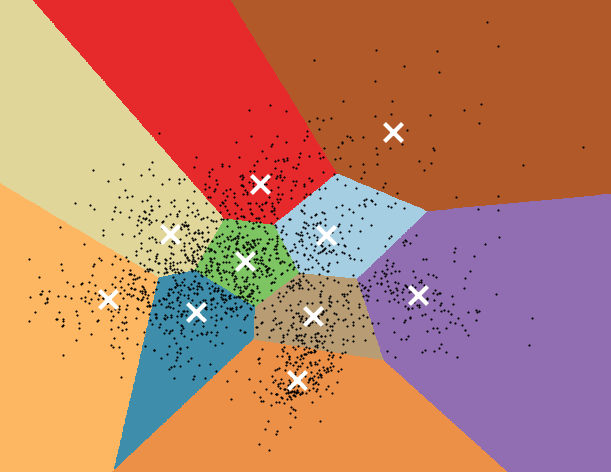
\includegraphics[width = 100mm]{kmeans}
	\caption{Esempio di Clustering utilizzando K-Means}
	\label{kmeans}
\end{figure}

\paragraph{HDBScan}
HDBScan � un algoritmo di Clustering che estende DBScan, rendendolo di tipo gerarchico.
\\
DBScan necessita di due parametri: $\epsilon$ e del numero minimo di elementi richiesti per formare un Cluster (minPts). Si comincia con un punto casuale che non � stato ancora visitato. Viene calcolato il suo $\epsilon$-vicinato, e se contiene un numero sufficiente di punti viene creato un nuovo raggruppamento. Se ci� non avviene, il punto viene etichettato come rumore, ovvero non viene associato ad alcun Cluster. � possibile che tale elemento rumore venga ritrovato in un $\epsilon$-vicinato sufficientemente grande e, quindi, inserito in un altro Cluster. Se un punto � associato ad un raggruppamento, allora anche tutti quelli nel suo $\epsilon$-vicinato sono parte del Cluster. Di conseguenza, tutti i punti trovati all'interno del suo $\epsilon$-vicinato sono aggiunti al Cluster, cos� come i loro $\epsilon$-vicini. Questo processo continua fino a quando il Cluster viene completato. Allora, un nuovo punto non visitato viene estratto e processato.

\begin{figure}[h]
	\centering
	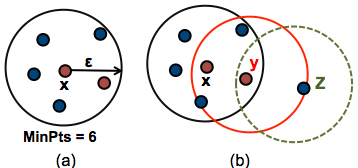
\includegraphics[width = 65mm]{dbscan}
	\caption{Principio su cui si basa DBScan}
	\label{dbscan}
\end{figure}

In HDBScan, invece, si parte in maniera simile a DBScan: lo spazio viene trasformato a seconda della densit� e viene effettuato su di esso una prossimit� a single-link. Invece di richiedere come input il parametro $\epsilon$, che viene usato da DBScan per considerare gli elementi del vicinato appartenenti al Cluster, viene creato un albero, il quale viene usato per selezionare i Cluster pi� stabili e persistenti. Viene solo richiesta la dimensione minima dei Cluster per determinare quali gruppi non devono essere considerati come Cluster, oppure per dividerli e formare nuovi Cluster.
\\
Questo algoritmo � molto efficace ed � pi� veloce sia di DBScan che di K-Means.

\section{Obiettivi della tesi}
Questa tesi ha due obiettivi:
\begin{enumerate}
	\item Capire se, combinando diverse rappresentazioni di cui una pagina Web si compone in uno spazio vettoriale al fine di applicare i tradizionali algoritmi di Clustering, vi � un miglioramento della qualit� dei Cluster prodotti.
	
	\item Verificare che, se analizzando la topologia del grafo del sito Web e dando pi� importanza a pagine vicino alla homepage, si ottengono risultati migliori rispetto all'approccio che analizza tutte le pagine come ugualmente importanti. La modifica applicata verr� discussa nella Sezione \ref{modifiedSkipgram}.
\end{enumerate}

\chapter{Stato dell'Arte}
\label{cap:capitolo2}
\documentclass[a4paper,12pt,oneside]{book}
\usepackage[usenames]{color} %usato per il colore
\usepackage{amssymb} %maths
\usepackage{amsmath} %maths
\usepackage[latin1]{inputenc}
\usepackage[pdftex]{graphicx} 
\usepackage{filecontents}
\usepackage[italian]{babel}
\usepackage{setspace}

\graphicspath{ {./../Immagini/} }

\begin{document}

\addtolength{\oddsidemargin}{+1,0cm} 
\addtolength{\evensidemargin}{+1,0cm} 
\onehalfspacing

%\tableofcontents
%\listoftables
%\listoffigures
%\newpage

% related work, dove � arrivata la scienza e i lavori che giustificano quello che ho fatto, il perch�
L'applicazione delle tecniche di Clustering su pagine Web non � un nuovo campo di ricerca. La maggior parte delle metodologie che si trovano in letteratura sono state usate per raggrupparle.
\\\\
Tuttavia queste ricerche sono state indirizzate sul Clustering di pagine provenienti da diversi siti Web, trascurando quelle di uno specifico sito. Gli hyperlink, infatti, hanno significati diversi in base al dominio di destinazione: se la pagina puntata si trova nello stesso sito Web, allora il collegamento avr� funzione di organizzazione dei contenuti; altrimenti, se la pagina di destinazione � esterna, avr� la funzionalit� di riferirsi a pagine che probabilmente avranno contenuti simili.
\\\\
Gli algoritmi di Clustering esistenti si classificano in quattro categorie in base alle informazioni usate per raggruppare le pagine Web:
\begin{itemize}
	\item \textbf{Algoritmi di Clustering basati sul contenuto testuale}. Questa tipologia di algoritmi considerano le pagine come dei documenti testuali. Questo � il caso di \cite{Zamir,Chehreghani,Haveliwala,Anami}, dove la distribuzione delle parole � usata per scoprire insiemi appropriati di pagine Web correlate. Il vantaggio di questo approccio � che molti strumenti di Clustering, basati sul modello dello spazio vettoriale, possono essere direttamente applicabili. Lo svantaggio � che questi algoritmi falliscono quando devono essere appresi modelli accurati, a causa della natura non controllata ed eterogenea dei contenuti delle pagine Web. 
	\\
	I tradizionali algoritmi di Clustering si basano sull'assunto che i documenti testuali condividono stili di scrittura consistenti, dando abbastanza informazioni contestuali, sono chiari e completamente non strutturati, sono indipendenti e identicamente distribuiti. Queste limitazioni sono pi� marcate per il Clustering di pagine Web di differenti siti. Infatti, le pagine aventi stesso argomento potrebbero essere contestualmente differenti: potrebbero avere un contenuto informativo simile inserito in elementi Web aventi diverse regole semantiche (i.e. tabelle o menu di navigazione) e differenti funzionalit� (i.e. link, pulsanti, immagini).
	\item \textbf{Algoritmi di Clustering basati sui Web log}. In questa tipologia si trovano algoritmi che analizzano ed estraggono informazioni a partire dai Web Log, che vengono usati per raggruppare pagine Web in funzione a schemi di comportamento degli utenti durante la navigazione in un determinato sito. In \cite{shahabi97knowledge} l'autore considera la cronologia di navigazione ed il tempo di visualizzazione di ogni pagina come informazioni per raggruppare i profili degli utenti. I cluster estratti possono essere usati per migliorare l'esperienza di navigazione degli utenti \cite{Crabtree}: cos� facendo, per esempio, � possibile migliorare la navigazione del sito Web di un dipartimento, differenziandola in base al profilo utente. Questa operazione di Clustering, tuttavia, pu� portare a difficolt�: ad ogni profilo utente potrebbero corrispondere cluster differenti di pagine Web.
	\item \textbf{Algoritmi di Clustering basati sulla struttura HTML}. Le pagine Web, a differenza dei documenti testuali, sono caratterizzate da propriet� strutturali come i tag HTML, che permettono di definire la loro rappresentazione strutturale. E' stato provato da \cite{crescenzi,bohunsky,lin,zhu} che l'informazione strutturale fornisce una differente e complementare rappresentazione rispetto a quella testuale. Questi tipi di algoritmi di Clustering hanno il vantaggio di considerare l'informazione strutturale e visuale inserita nei tag HTML, che viene ignorata dall'approccio testuale. I tag HTML sono i responsabili della visualizzazione dei dati all'interno di una pagina Web. Per questo � possibile avere pagine aventi lo stesso tipo di semantica (e.g. pagine di professori) ma codificate e visualizzate in maniera differente. Per esempio, i dati strutturati inseriti in tabelle (aventi come tag HTML $<$table$>$) oppure in liste (aventi come tag HTML $<$ul$>$) avranno una simile visualizzazione. Questo abbassa la qualit� dei cluster generati.
	\\
	Per risolvere questa sfida, gli autori di \cite{crescenzi,bohunsky} propongono di usare l'informazione associata ai tag HTML. In \cite{bohunsky} viene effettuato un processo di Clustering basandosi solo sulle propriet� visuali delle pagine Web. L'obiettivo di questo approccio � quello di raggruppare le pagine Web che hanno una visualizzazione simile, trascurando il contenuto e la struttura HTML. In \cite{crescenzi} il layout e le propriet� visuali associati ai tag HTML vengono usati per caratterizzare la struttura dell'intera pagina Web, mentre le collezioni di hyperlink vengono considerate per trovare pagine avente una rappresentazione strutturale simile.
	\item \textbf{Algoritmi di Clustering basati sulla struttura ad hyperlink}. Anche la struttura ad hyperlink che interconnettono le pagine Web caratterizzano le loro propriet� strutturali. Gli algoritmi basati sulla struttura ad hyperlink lavorano su una collegata collezione di pagine Web. L'idea di base � che quando due pagine web sono connesse tramite un link esiste una relazione tra le due. Da qui sar� possibile effettuare il Clustering. In generale, questi metodi \cite{Cristo2003} usano solo link diretti tra le pagine e, da questi, vengono usate/definite alcune misure di similarit�, come la somiglianza bibliografica \cite{kessler} e le co-citazioni \cite{small}.
	\\
	In \cite{fisher}, l'autore spiega come questa tipologia di algoritmi di Clustering lavorano bene quando la struttura ad hyperlink � densa e senza link rumore. Essi restituiscono risultati di bassa qualit� per pagine Web aventi un numero insufficiente di link, sia che portino a pagine appartenenti allo stesso sito Web, sia che puntino a pagine di siti differenti. Inoltre, non tutti i link hanno stessa importanza nel processo di Clustering: le pagine sono spesso arricchite di link rumore come gli short-cut hyperlink (i link scorciatoia). Per superare questo problema, molti algoritmi combinano le informazioni ricavate dal contenuto con quelle dei link \cite{lin,He01webdocument,Modha,Wang,Drost2006,Angelova}.
	\\
	Inoltre, in \cite{He01webdocument} l'autore ha risolto il problema dei link rumore considerando solo gli hyperlink tra pagine web di argomento simile e co-citate. Successivamente, � stato applicato un tradizionale algoritmo di Clustering basato sul partizionamento del grafo. In particolare, � stato assegnato un peso che combina la similarit� di contenuto e la co-citazione per ogni arco $(i, j)$, dove $i$ e $j$ sono le pagine collegate del grafo del sito Web. Il metodo ha due principali limitazioni: \textit{i}) le informazioni testuali vengono usate solo per definire i pesi dei link, di conseguenza due pagine Web condivideranno le stesse propriet� distribuzionali, ma, avendo una similarit� testuale bassa, non potranno essere inserite nello stesso cluster; \textit{ii}) l'algoritmo di Clustering del grafo � NP-hard, ovvero � altamente complesso in termini di computazione.
	\\
	In \cite{lin}, l'autore propone una misura di similarit� ottenuta combinando la somiglianza di tipo testuale, di co-citazione, di bibliografia e della struttura ad hyperlink che interconnettono pagine dello stesso sito Web. In questo modo, due pagine che hanno una similarit� di struttura ad hyperlink appariranno pi� volte all'interno della collezione dei link.  Le combinazioni delle varie similarit�, ancora oggi, sono ancora un problema aperto.
\end{itemize}

\section{Altre metodologie di Clustering}
Gli algoritmi di Clustering basati sulla struttura ad hyperlink considerano solo relazioni dirette tra i vicini, senza analizzare la struttura globale del grafo del sito Web. In \cite{gornerup,zhou,tang2015line} gli autori sostengono che la similarit� tra i nodi di due grafi pu� essere rappresentata in termini di somiglianza dei loro rispettivi contesti: in altri termini, come condividono i nodi vicini.
\\
In \cite{zhou} viene proposto un algoritmo di Clustering che si concentra sulla struttura topologica di un grafo e sulle propriet� dei nodi, che possono essere testuali o relazionali. Un insieme di nodi ed archi attributi vengono aggiunti al grafo originale. Cos� facendo, la similarit� degli attributi � trasformata in base alla vicinanza dei vertici nei grafi: due vertici che condividono un attributo sono collegati da uno di tipo attributo. Nonostante l'algoritmo possa combinare sia le informazioni strutturali che di contenuto, usando una comune rappresentazione, non pu� essere utilizzato a dati che hanno valori numerici (e.g. tf-idf) o attributi categorici aventi un gran numero di valori distinti.
\\
In \cite{tang2015line} viene proposto un metodo di embedding chiamato Line. Questa metodologia sfrutta la rete neurale per generare una rappresentazione vettoriale densa e a bassa dimensionalit� dei nodi del grafo. Line \cite{tang2015line} ottimizza una funzione che incorpora le strutture locali e globali della rete. Una limitazione di questa metodologia � che vengono ignorati i nodi attributo (e.g. contenuto testuale). Di conseguenza, l'operazione di Clustering basata su embedding generati da Line potrebbero essere difficoltosi in grafi senza sufficienti hyperlink interni ed esterni, ma caratterizzati da ricchi contenuti testuali.

\subsection{Combinazione di embeddings}
Recenti sperimentazioni hanno esaminato vari approcci di generazione di embedding per capire i punti di forza e le debolezze di ognuno. Altre aree di ricerca del Machine Learning hanno scoperto che, combinando varie tecniche, � possibile ottenere risultati eccellenti.
\\
In questo contesto, gli autori di \cite{garden} hanno esplorato varie tipologie di composizioni di embedding, dimostrando che i vari metodi di combinazione dei vettori degli embedding possono produrre spazi vettoriali ibridi che forniscono risultati aventi una bont� significativa. Nello specifico, hanno cercato di capire se si ottengono risultati migliori  effettuando una semplice addizione o una concatenazione tra i vettori. Gli spazi vettoriali sono stati prodotti da due algoritmi differenti di Machine Learning:
\begin{itemize}
	\item \textbf{DVRS}. E' un metodo per generare rappresentazioni vettoriali semantiche. Ogni parola � rappresentata da due vettori: un vettore ambientale fisso $e(i)$ viene generato casualmente assegnando ad ogni elemento del vettore un valore compreso tra $[-1,1)$; il vettore lessicale $l(i)$ cattura, invece, il significato della parola, che viene aggiornato durante l'apprendimento. Una volta che il documento viene processato, il vettore lessicale di ogni parola viene aggiornato in base sia al contesto di paragrafo $c(k)$, sia al contesto di ordine della frase $o(k)$. Rispettivamente:
	\begin{equation}
		c(k) = \sum_{i=1}^{n} e(i), i \neq k
	\end{equation}
	\begin{equation}
		o(k) = \sum_{j=-4}^{4} s(j) * e(k + j)
	\end{equation}
	dove $j \neq 0$ e $0 < (k + j) \leq n $.
	\item \textbf{Word2Vec}. E' un algoritmo di Word Embedding che trasforma parole in Feature Vectors. Per approfondimenti, vedere la Sezione \label{word2vec}.
\end{itemize}
I risultati riportati da \cite{garden} mostrano come la combinazione dei vettori di DVRS e di Word2Vec porta ad un incremento della bont� dei risultati.

\bibliographystyle{plain}
\bibliography{./../Bibliografia}                % database di biblatex 

\end{document}

\chapter{Pianificazione della sperimentazione}
\label{cap:capitolo3}
Il Clustering delle pagine di un sito Web � un processo fondamentale nel Web Mining per valutare l'interazione tra le pagine, organizzare i contenuti del sito e capire come questo sia stato strutturato. 
\\
Una pagina Web � composta da varie propriet� che la caratterizza e la diversifica dalle altre. Nello specifico, una pagina di un sito � composta da:
\begin{itemize}
	\item \textbf{Rappresentazione testuale}. Il testo � una componente fondamentale di una pagina Web, poich� ha come scopo il trasferimento dell'informazione: durante la navigazione, l'utente estrapola conoscenza semplicemente leggendo il contenuto testuale delle pagine che visita.
	\item \textbf{Rappresentazione visuale}. Quando una pagina Web viene renderizzata da un browser, viene applicato uno stile di formattazione visuale, chiamato CSS, che definisce gli elementi della pagina Web come contenitori rettangolari che sono disposti o uno dopo l'altro o annidati tra loro formando un albero chiamato \texttt{Rendered Box Tree}. L'albero in questione � differente dalla struttura della pagina definita dai tag HTML poich� una pagina pu� essere ricca di elementi invisibili, come il tag $<$head$>$ o da elementi aventi come stile $display:none$. Inoltre, la generazione del rendered box tree richiede l'esecuzione di codice JavaScript e CSS.
	\item \textbf{Rappresentazione strutturale}. Questa � composta da elementi Web inscritti in tag HTML ed organizzata ad albero. I tag HTML possono essere applicati a porzioni di testo, hyperlink e dati multimediali per fornire loro un significato ed una renderizzazione differente della pagina da parte del browser.
\end{itemize}
Attualmente, gli esistenti algoritmi di Clustering sfruttano le propriet� delle pagine Web per assegnare, ad ognuna di esse, un gruppo. Ma l'utilizzo di queste caratteristiche avviene in maniera indipendente, poich� esse sono difficili da combinare.
\\\\
In questa tesi si approfondiscono tecniche e metodologie per sfruttare a pieno le propriet� delle pagine di un sito Web per permettere la generazione di cluster di pagine pi� omogenei. Si � cercato di capire come combinare queste informazioni in un singolo spazio vettoriale.
\\\\
Nelle sottosezioni che seguono si descrivono i passi che sono stati effettuati per pianificare ed eseguire la metodologia. Nello specifico, sono state applicate tre operazioni principali:
\begin{itemize}
	\item \textit{Crawling delle pagine Web}
	\item \textit{Costruzione del Dataset}
	\item \textit{Clustering delle pagine Web}
\end{itemize}

\section{Web Crawling}
Le propriet� che caratterizzano le pagine Web rendono complicato il processo di estrazione di informazioni, soprattutto nel caso in cui i contenuti vengono generati dinamicamente. Per analizzare i contenuti della rete e delle pagine Web si utilizza un software automatizzato chiamato Web Crawler. Tipicamente, questo programma viene usato per molti altri scopi, come l'indicizzazione di pagine Web. I motori di ricerca sfruttano tali indici per aumentare l'efficienza delle interrogazioni che gli utenti effettuano durante la navigazione.
\\
La ragione principale dell'uso dei crawler � che il World Wide Web non � un contenitore centralizzato: pu� essere visto, infatti, come un insieme di siti Web che forniscono differenti servizi.
\\\\
L'algoritmo di crawling � relativamente semplice: dato un insieme di URL di pagine Web, vengono scaricate tutte le pagine associate all'indirizzo URL, estratti gli hyperlinks e, iterativamente, scaricate le pagine associate a questi link. Il loro contenuto verr� analizzato e salvato per essere successivamente indicizzato. Nonostante l'apparente semplicit� di questo algoritmo, l'attivit� di Web crawling � caratterizzata da obiettivi inerenti \cite{crawling}:
\begin{itemize}
	\item \textbf{Scalabilit�}. Il Web � molto grande e in continua evoluzione. I crawler che cercano una copertura ampia ed aggiornata devono raggiungere throughput (prestazioni) estremamente alti. Per riuscirci, bisogna risolvere problematiche ingegneristiche complesse. I moderni motori di ricerca impiegano migliaia di computer e decide di collegamenti di rete ad alta velocit�.
	\item \textbf{Compromessi di selezione dei contenuti}. Persino i crawler con un alto throughput non sono in grado di scandire l'intero Web o tenere traccia di tutti i cambiamenti. Per questo, il processo di crawling viene effettuato in maniera selettiva con un attento e controllato ordine. Gli obiettivi sono di acquisire velocemente i contenuti aventi un alto valore, di assicurare la copertura di tutti i contenuti scelti, di ignorare quelli a bassa qualit�, irrilevanti, ridondanti e dannosi e di mantenerli aggiornati. Il Crawler deve rispettare alcuni vincoli come il numero massimo di visite per sito e le pagine da scartare durante l'analisi.
	\item \textbf{Obblighi sociali}. I crawler dovrebbero essere dei "buoni cittadini" del Web: non devono sovraccaricare i siti che scandiscono. Infatti, senza i giusti meccanismi, un throughput alto pu� inavvertitamente provocare un attacco Denial of Service (DOS), sovraccaricando il server Web rendendolo inaccessibile.
	\item \textbf{Avversari}. Alcuni siti Web cercano di iniettare contenuti inutili o fuorvianti nel corpus assemblato dai crawler. Questo comportamento � spesso motivato da incentivi finanziari, per esempio per indirizzare male il traffico verso siti commerciali.
\end{itemize}

\begin{figure}[h]
	\centering
	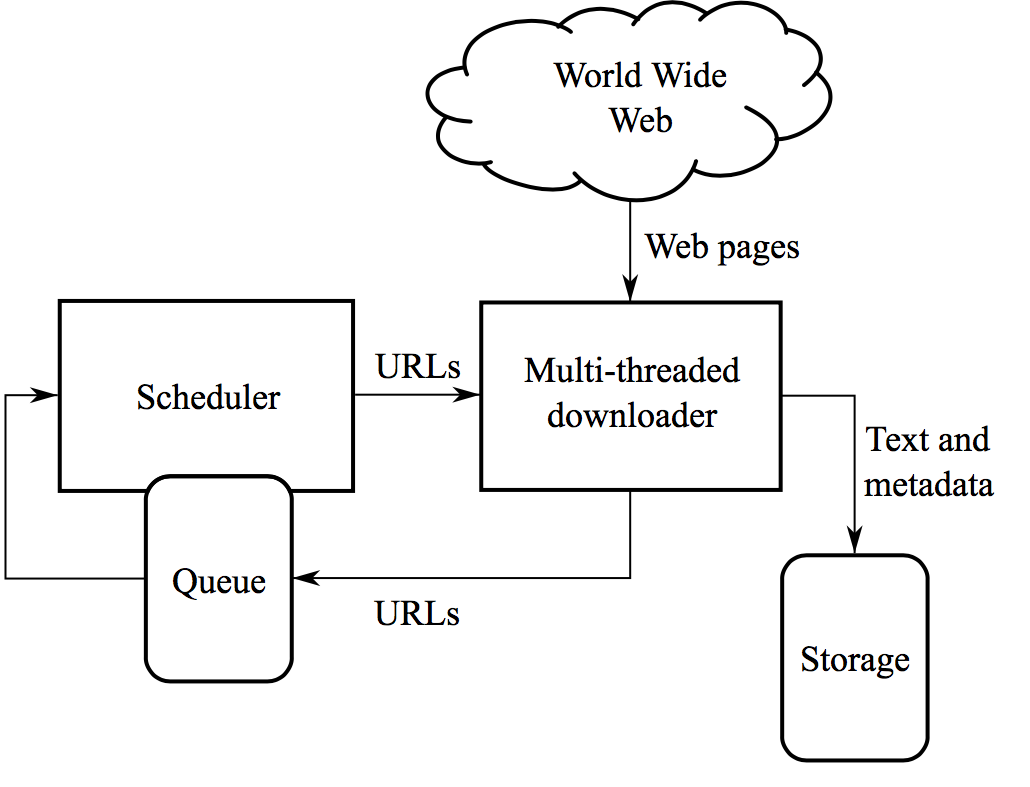
\includegraphics[width = 100mm]{WebCrawlerArchitecture}
	\caption{Architettura di un web crawler}
	\label{crawlerarchitecture}
\end{figure}

\subsection{Crawling delle pagine di un sito Web}
Ai fini sperimentali � stato utilizzato un Web Crawler che estrae gli hyperlink di un sito Web per effettuare successivamente l'operazione di Clustering delle pagine associate a tale sito.
\\\\
Un sito Web pu� essere formalmente descritto come un grafo orientato $G = (V, E)$, dove $V$ � l'insieme delle pagine appartenenti al sito ed $E$ � l'insieme degli hyperlink. In molti casi, la homepage $h$ di un sito rappresenta il punto di inizio, tecnicamente espresso come un grafo orientato radicato (albero), che consente l'esplorazione da parte degli utenti.
\\\\
Il grafo del sito Web pu� essere ricco di link rumore (e.g. hyperlink scorciatoia) che non sono rilevanti nel processo di Clustering \cite{crescenzi} e vengono esclusi dal Crawling. In pi�, la struttura del sito Web � codificata in sistemi di navigazione che offrono una visuale della sua organizzazione. Questi sistemi vengono implementati come collezioni di link che hanno lo stesso dominio e condividono il layout e le propriet� visuali.

\newpage

\begin{algorithm}[h]
	\caption{crawlingWebsite(homepage)}
	
	\begin{algorithmic}
		\State \textbf{Input:} URL homepage
		\State \textbf{Output:} Set$<$(URL, URL)$>$ E; Set$<$(URL, String)$>$ V
		\State $frontier \gets Set()$
		\State $Q \gets Queue(homepage)$
		
		\Repeat
			\State $currentPage \gets Q.dequeue()$
			\State $text \gets currentPage.getText()$
			\State $V.add((currentPage, text))$
			\State $webLists \gets extractWebLists(currentPage)$
			
			\For{\textbf{each} $a \in b$}
				\State $pagesToAnalyze \gets list.filterNot(page \to frontier.contains(page))$
				\State $Q.enqueue(pagesToAnalyze$
				\State $frontier.add(pagesToAnalize)$
				
				\For{\textbf{each} $u \in pagesToAnalyze$}
					\State $E.add((currentPage, u))$
				\EndFor
			\EndFor
		\Until{$!Q.empty()$}
		\State \textbf{return} $(V, E)$
	\end{algorithmic}
\end{algorithm}

La soluzione utilizzata per indicizzare un sito Web � stata quella di sfruttare il concetto di \textbf{lista Web}.
\\
Per definizione, una lista Web � una collezione di due o pi� elementi web che hanno struttura HTML simile, visualmente adiacenti ed allineati sulla pagina renderizzata. Questo allineamento pu� essere visto sia lungo l'asse x (i.e. una lista verticale), sia lungo l'asse y (i.e. una lista orizzontale), o ancora in maniera mista (i.e. griglia).

\newpage

\begin{figure}[h]
	\centering
	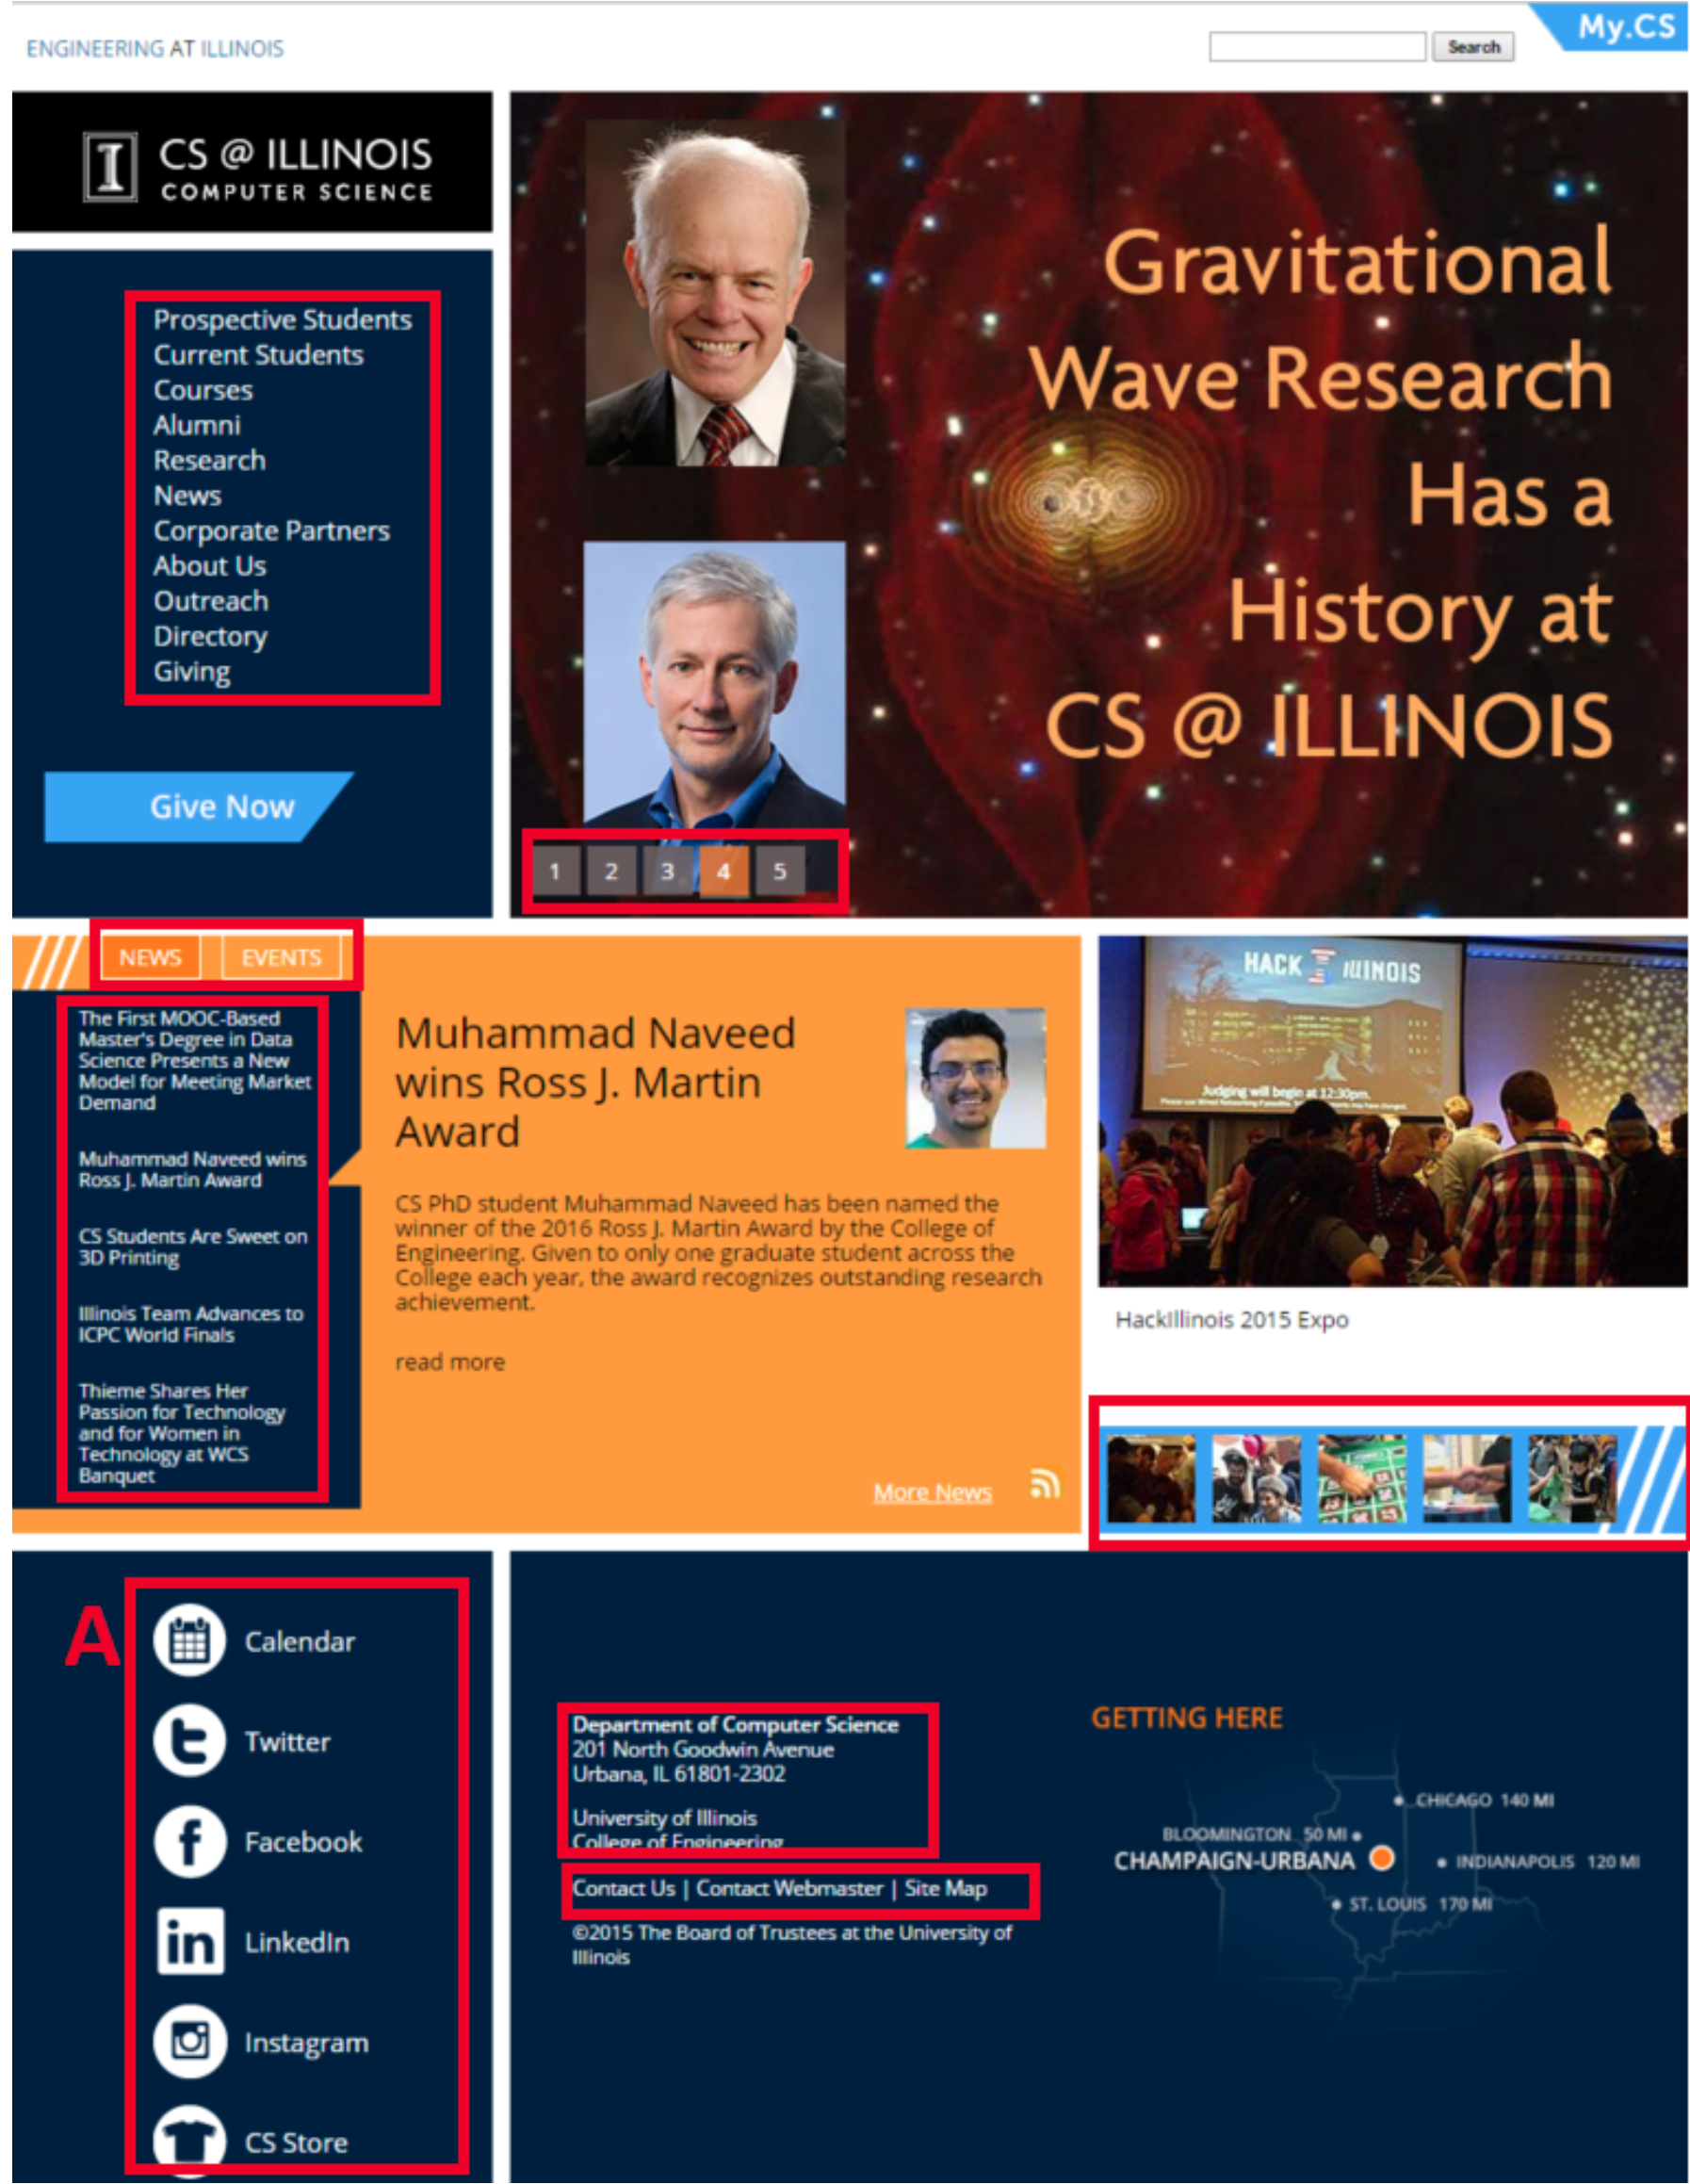
\includegraphics[width = 100mm]{weblistexample}
	\caption{Esempio di liste Web}
	\label{weblistfigure}
\end{figure}

In Figura \ref{weblistfigure} vengono mostrate le liste Web, usate per guidare il processo di Crawling.

\subsection{Normalizzazione degli URL}
Una volta effettuato il processo di Crawling ed estratti gli URL, si � proceduto alla normalizzazione degli stessi.
\\
Questo � un processo in cui gli URL vengono modificati e standardizzati in maniera consistente. Il suo obiettivo � poter determinare se due URL, che sono sintatticamente differenti, possono essere equivalenti.
\\
I Crawler effettuano un qualche tipo di normalizzazione degli URL in modo da evitare che il processo di Crawling non vada ad analizzarli pi� volte.
\\\\
\texttt{http://www.facebook.com/}
\\
\texttt{facebook.com/}
\\\\
\texttt{http://208.77.188.166/}
\\
\texttt{http://www.example.com/}
\\\\
La normalizzazione di URL, come si evince dagli esempi sopra riportati, pu� comprendere sia la rimozione del protocollo ("http://") e della stringa "www", oppure la sostituzione dell'indirizzo IP con il nome del dominio. E' bene sottolineare come le due coppie in analisi puntino a due siti Web, rispettivamente \textit{Facebook} ed \textit{example}.
\\
Ci sono diverse modalit� di normalizzazione che possono essere effettuate, fra cui la conversione degli URL in minuscolo e la rimozione del "." e ".." per portare gli URL da assoluti a relativi, aggiungere slash finali al componente di percorso non vuoto.
\\\\
Per la sperimentazione si � scelto di normalizzare gli URL eliminando la dicitura del protocollo ("http://" o "https://"), del "www" e dello slash finale.

\section{Costruzione del dataset}
Il crawler, a seguito dell'analisi del sito, ha prodotto un grafo delle pagine Web ed il contenuto testuale di ogni pagina esplorata. Il grafo del sito Web servir� per generare le sequenze attraverso i Random Walks.
\\
Per ridurre lo spazio in memoria e i tempi di elaborazione, � stato associato ad ogni URL un codice univoco, che permette l'identificazione dello stesso.

\subsection{Random Walks}
Un Random Walk, o passeggiata aleatoria, � la formalizzazione dell'idea di effettuare passi successivi in direzioni casuali. Dal punto di vista matematico � il processo stocastico pi� semplice, ovvero quello markoviano, nel quale la probabilit� che determina il passaggio ad uno stato, dipende solo dallo stato immediatamente precedente, e non dal come si � giunti a tale stato.
\\\\
In una passeggiata aleatoria monodimensionale si studia il moto di una particella puntiforme vincolata a muoversi lungo una retta nelle due direzioni consentite. Ad ogni movimento, questa si sposta a caso o a destra, con una probabilit� fissata \textbf{p}, oppure a sinistra, con una probabilit� \textbf{1 - p}, ed ogni passo � di lunghezza uguale e indipendente dagli altri.

\begin{figure}[h]
	\centering
	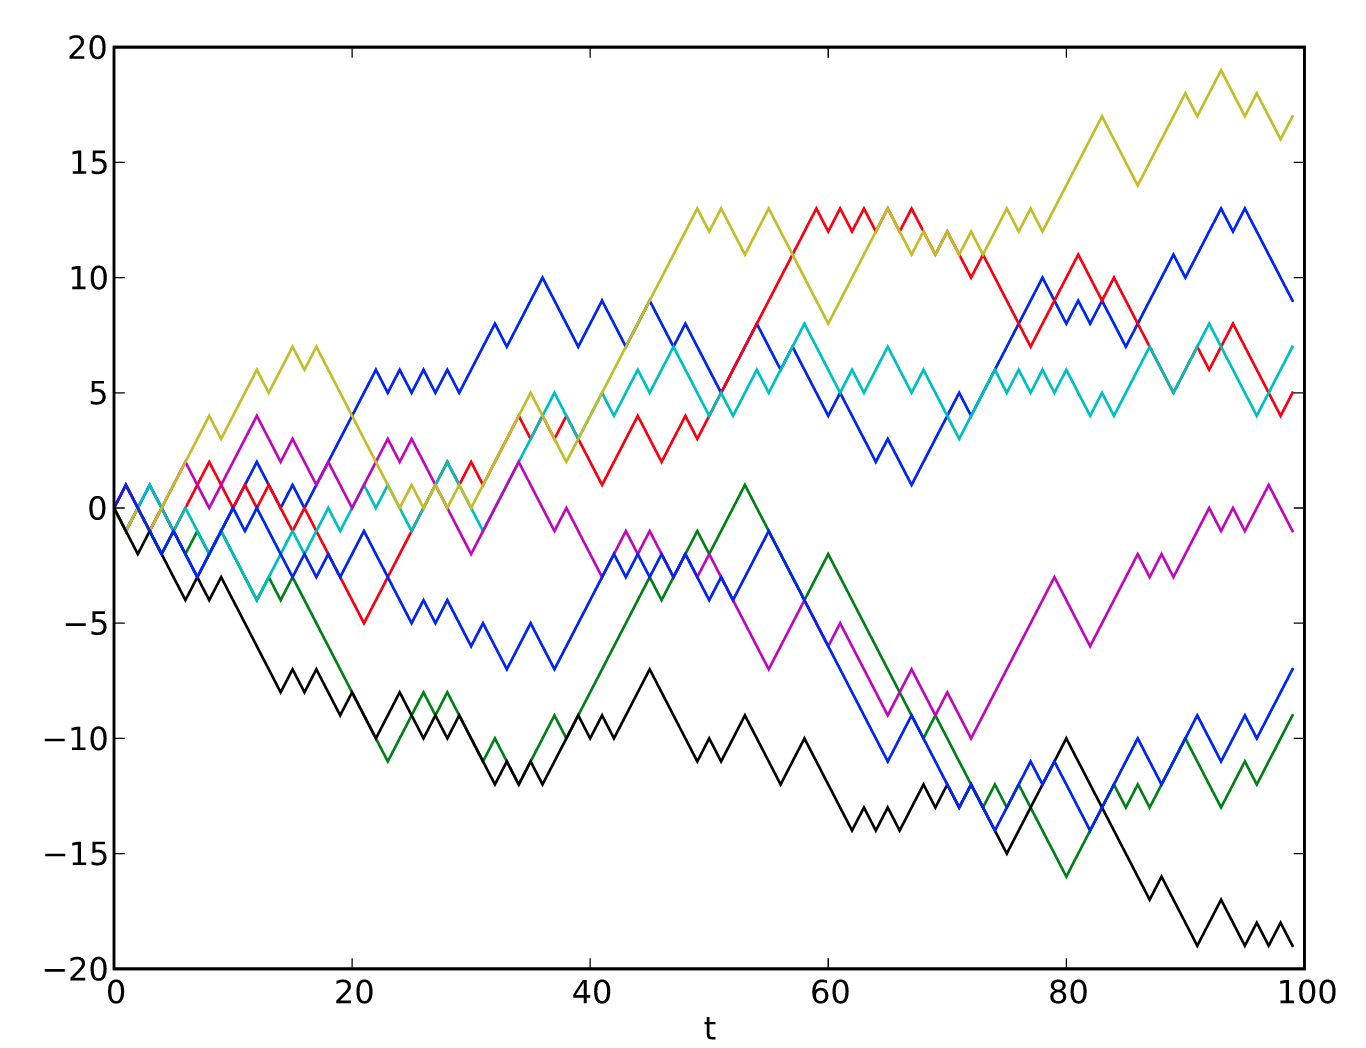
\includegraphics[width = 120mm]{randomwalkmono}
	\caption{Esempio di otto Random Walks in una dimensione}
	\label{randomwalkmono}
\end{figure}

In una passeggiata aleatoria bidimensionale si studia il moto di una particella vincolata a muoversi sul piano spostandosi casualmente ad ogni passo a destra, a sinistra, in alto o in basso con probabilit� \textbf{1/2}. Praticamente, ad ogni passo, la particella pu� compiere un movimento lungo una delle quattro diagonali con probabilit� \textbf{1/4}. Ma qual � la probabilit� che la particella torni al punto di partenza? In questo caso, la particella, che � libera di camminare casualmente con uguale probabilit� nelle quattro direzioni, torner� infinite volte al punto di partenza.

\begin{figure}[h]
	\centering
	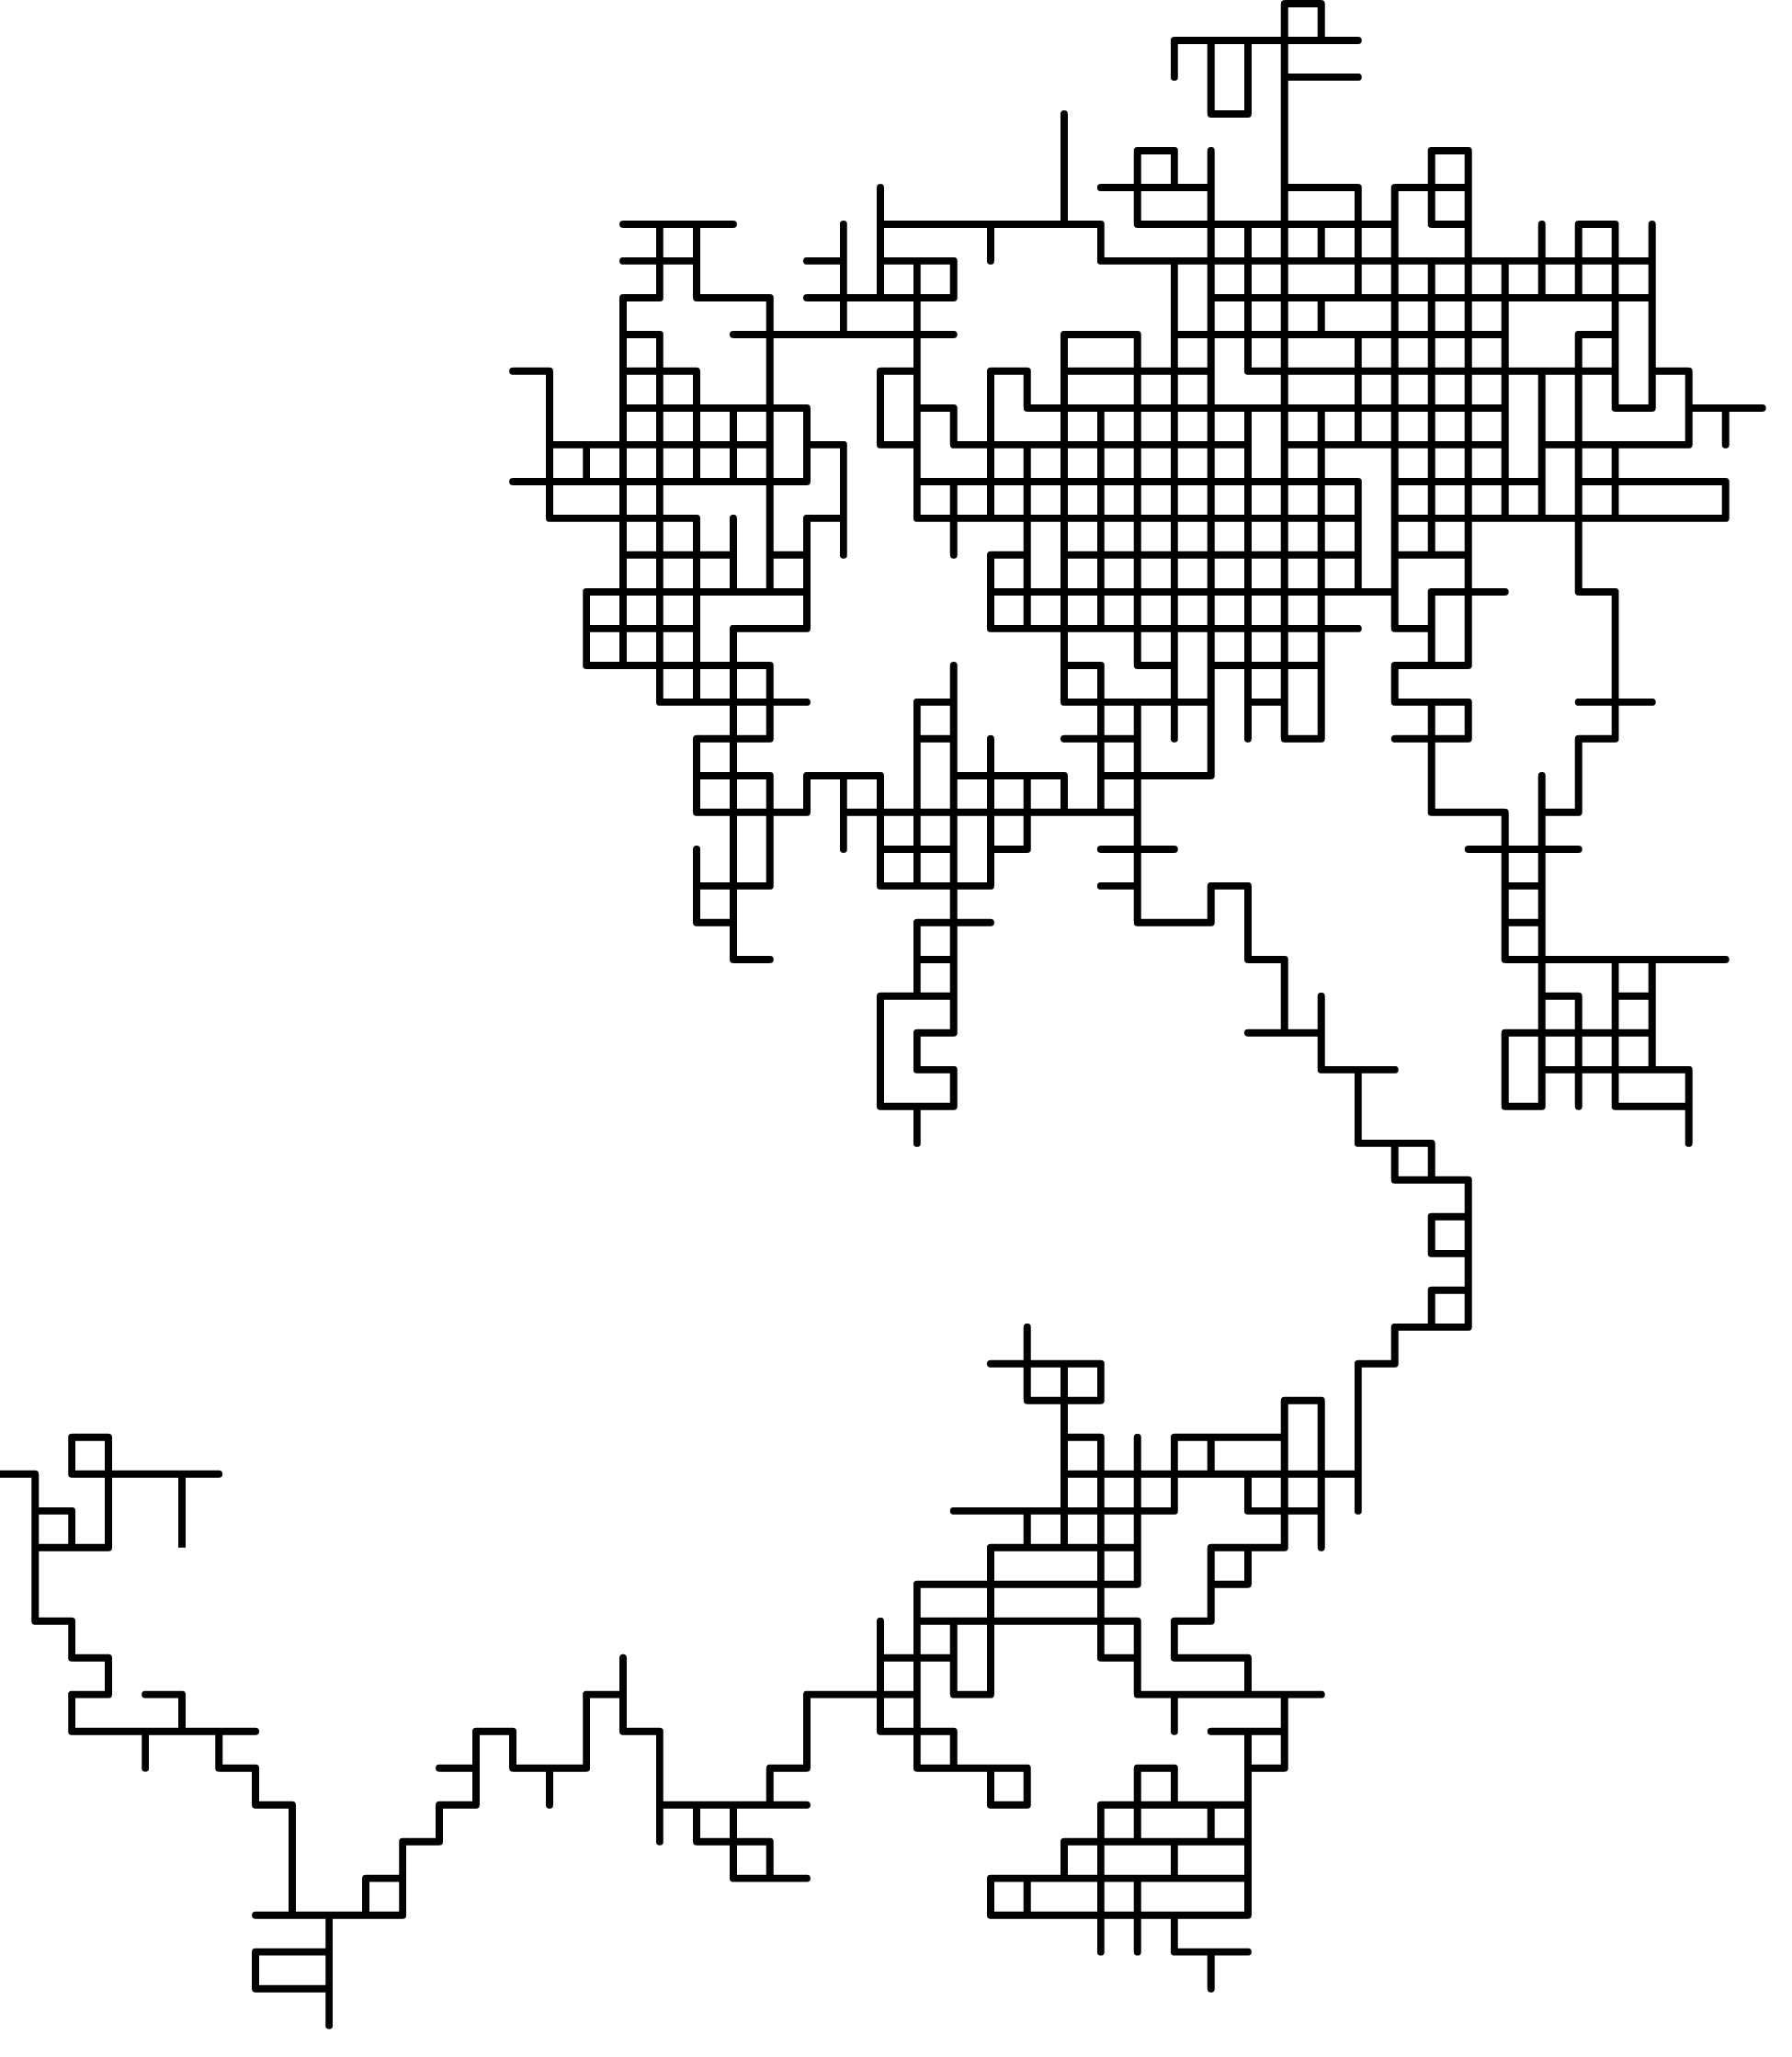
\includegraphics[width = 120mm]{randomwalkbi}
	\caption{Esempio di Random Walks in due dimensioni}
	\label{randomwalkbi}
\end{figure}

In una passeggiata aleatoria tridimensionale si studia il moto di una particella vincolata a muoversi nello spazio spostandosi casualmente ad ogni passo a destra, a sinistra, in alto, in basso, in su o in gi� con probabilit� \textbf{1/2}. In pratica ad ogni passo pu� compiere un movimento lungo una delle otto diagonali con probabilit� \textbf{1/8}. Come nel caso precedente, � stata calcolata la probabilit� che la particella torni prima o poi al punto di partenza ed � pari a \textbf{0,239}.

\begin{figure}[h]
	\centering
	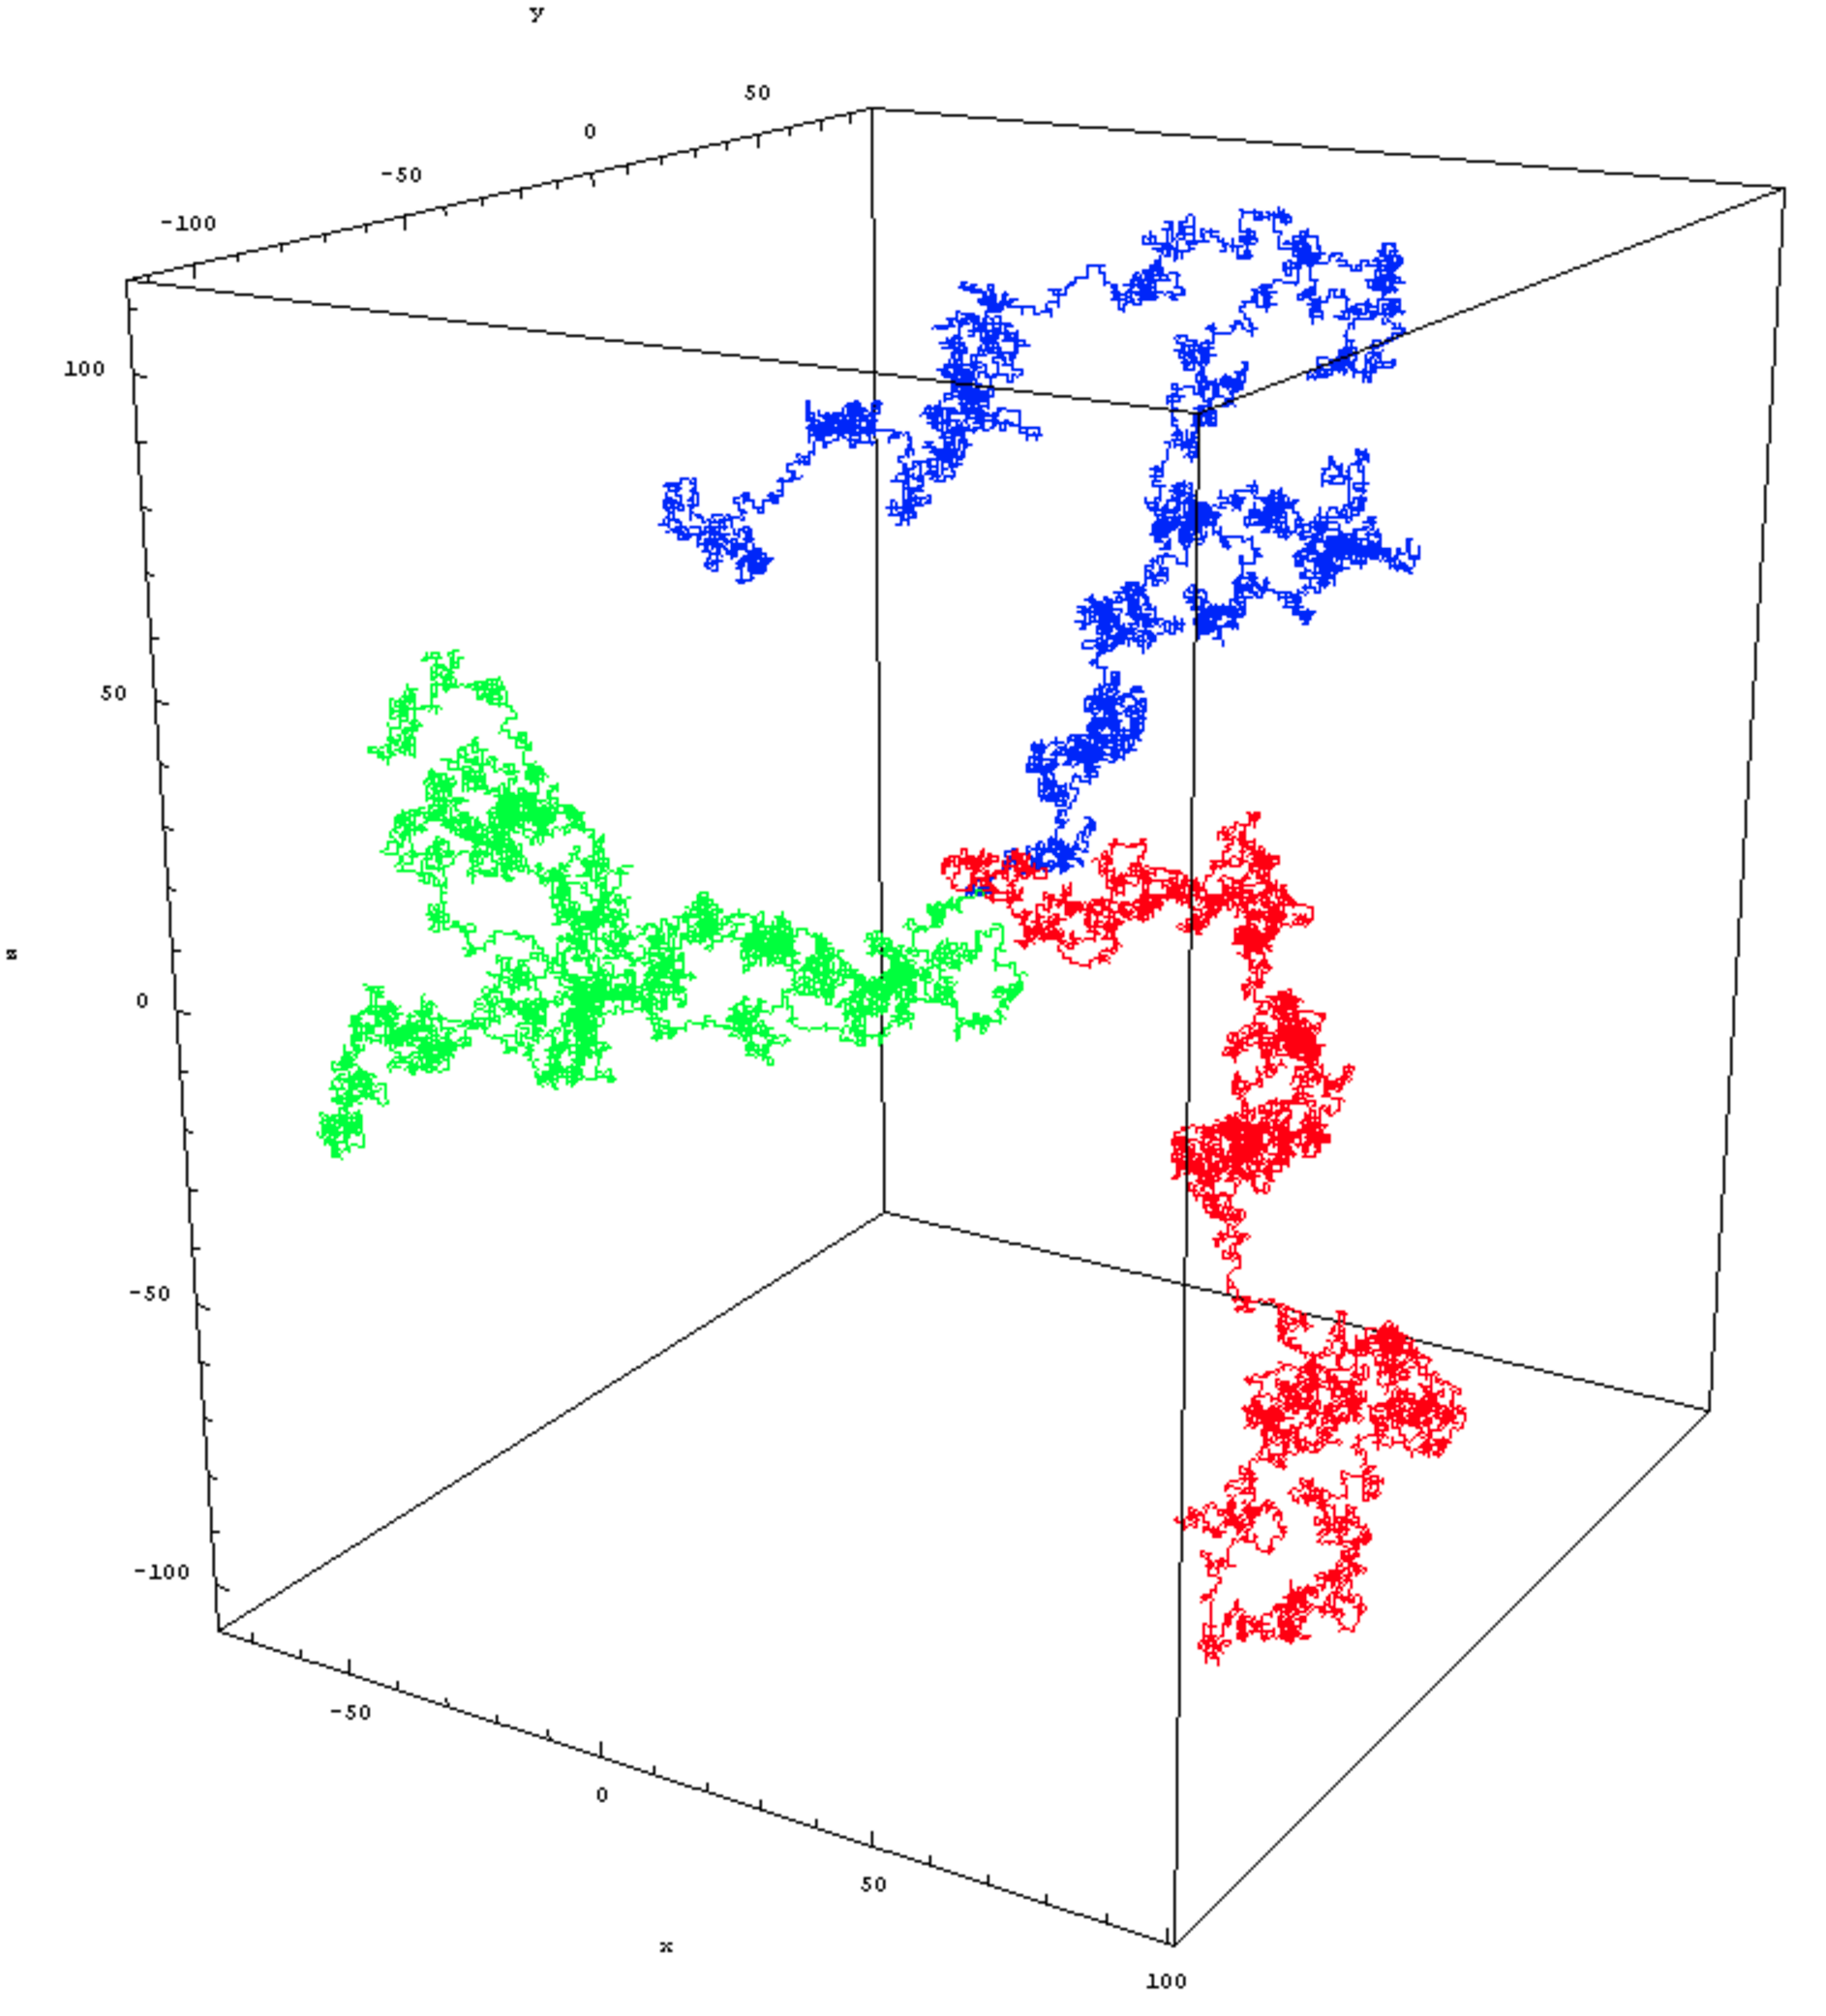
\includegraphics[width = 120mm]{randomwalktri}
	\caption{Esempio di Random Walks in tre dimensioni}
	\label{randomwalktri}
\end{figure}

Il concetto di Random Walk � stato applicato nei campi pi� disparati, alcuni dei quali sono:
\begin{itemize}
	\item \textbf{Economia finanziaria}. I Random Walk sono stati usati per modellare i prezzi delle azioni sui mercati azionari, tassi di cambio di moneta e materie prime.
	\item \textbf{Genetica}. Descrivono le propriet� statistiche della deriva generica, ovvero una componente dell'evoluzione di una specie dovuta a fattori casuali, che pu� essere studiata con metodi statistici.
	\item \textbf{Fisica}. Usati come modelli semplificati per studiare il moto browniano, ovvero il moto della particelle presenti in fluidi che � osservabile al microscopio.
	\item \textbf{Ecologia matematica}. Usati per descrivere i movimenti dei singoli animali, i processi di diffusione della materia, o ancora per la dinamica della popolazione. Quest'ultimo studia i cambiamenti del numero di individui, della densit� e della struttura di una o diverse popolazioni. Inoltre analizza i processi biologici e ambientali che influenzano queste trasformazioni.
	\item \textbf{Informatica}. Usati per stimare la dimensione del Web, ovvero il numero di pagine e di siti che fanno parte del World Wide Web.
\end{itemize}

\subsection{Generazione delle sequenze}
Una passeggiata aleatoria sulla struttura ad hyperlink di un sito Web si basa sull'idea che le connessione tra nodi (i.e. le pagine del sito) presentano delle informazioni latenti circa la loro correlazione. Per catturarle si � deciso di utilizzare un Random Walker, una componente incaricata di effettuare le passeggiate aleatorie sul grafo di un sito Web. Questa scelta � motivata dal fatto che le metodologie selettive per esplorare un sito Web, che derivano dalla teoria dei grafi, prevedono l'esplorazione di tutte le possibili opzioni per arrivare alla soluzione. Ma tali tecniche sono difficilmente computabili in quanto ricadono nella classe di complessit� NP-completa.
\\
Il Random Walker, anche se permette di avere buone approssimazioni nell'esplorazione del grafo del sito, presenta una problematica: potrebbe capitare che la pagina che sta analizzando non presenta link al suo interno. La soluzione pi� diffusa � quella di effettuare un "salto" verso una qualsiasi altra pagina. Nel nostro caso, invece, dato che le sequenze da generare devono avere una lunghezza massima fissata prima della generazione, se l'attraversatore casuale incontra una pagina priva di hyperlink allora si blocca semplicemente. La sequenza finale quindi, risulter� pi� piccola. Questa scelta � stata presa poich� l'informazione cercata nasce da percorsi reali di navigazione e non vi � la necessit� di una lunghezza obbligatoria da rispettare, in quanto le sequenze possono essere viste come frasi di un testo, dove le parole sono gli URL.

\begin{algorithm}[h]
	\caption{rwrGeneration(rwrLength, dbLength, G, $\alpha$)}
	\label{rwrGeneration}
	
	\begin{algorithmic}
		\State \textbf{Input:} int rwrLength \Comment{numero di passi massimo}
		\State \textbf{Input:} int dbLength \Comment{numero di frasi}
		\State \textbf{Input:} Graph G \Comment{il grafo del sito Web}
		\State \textbf{Input:} float $\alpha$
		\State \textbf{Output:} List$<$List$<$URL$>$$>$ randomWalks
		
		\For{\textbf{each} $i \in Range(0, dbLength)$}
			\State $w \gets List()$
			\State $w[0] \gets G.getRandomVertex()$

			\For{\textbf{each} $j \in Range(1, rwrLength)$}
				\State $\lambda \gets Math.random()$
				\If{$\lambda > \alpha$}
					\State $w[j] \gets G.getRandomOutlink(w[j-1])$
				\Else
					\State $w[j] \gets w[0]$
				\EndIf
			\EndFor
			
			\State $randomWalks.add(w)$
		\EndFor
		
		\State \textbf{return} $randomWalks$
	\end{algorithmic}
\end{algorithm}

Per motivi di sperimentazione sono stati implementati tre tipi diversi di Random Walk, utilizzabili modificando i parametri di esecuzione dell'Algoritmo \ref{rwrGeneration}.

\paragraph{Random Walk standard}
Il caso standard prevede che si parta da un nodo casuale del grafo e si segua ogni volta un arco a caso fra quelli disponibili, fino al raggiungimento della lunghezza prefissata o all'impossibilit� di proseguire.

\paragraph{Random Walk con partenza da homepage}
Con quest'altra modalit� si ha una partenza fissata. Si parte, quindi, da un nodo prefissato del grafo, generalmente la homepage del sito Web in analisi, in modo da esplorare pi� percorsi possibili.

\paragraph{Random Walk attraverso le Liste}
Questo � il caso in cui si pu� eseguire uno delle due tipologie di Random Walks viste in precedenza, ma aventi il vincolo delle liste: l'algoritmo, quindi, operer� solo su un sottoinsieme di quello prodotto dalla metodologia scelta.

\section{Modifica dell'implementazione di Word2Vec}
Un aspetto particolare preso in considerazione in questa tesi � stato quello di chiedersi se, modificando in maniera opportuna l'algoritmo di Word Embedding Word2Vec, si potesse avere un miglioramento nel processo di Clustering delle pagine del grafo del sito Web in analisi.
\\
Per rispondere a questa domanda, si � deciso di analizzare e modificare il modello di apprendimento di Word2Vec Skip-Gram della libreria \texttt{deeplearning4j}. Questo modello consiste nel predire il contesto a partire da una parola. Per una argomentazione pi� approfondita si veda la Sezione \ref{word2vec}.
\\
La modifica di Skip-Gram consiste nel limitare l'apprendimento dell'algoritmo in maniera tale che venga analizzato solo il contesto sinistro, data una parola. E' importante sottolineare, inoltre, come questo modello sia stato ottimizzato con un valore chiamato \textbf{b}, che permette di aumentare o diminuire la finestra di contesto, dando pi� importanza alle parole pi� vicine a quella in analisi.
\\
Per la sperimentazione sono stati prodotti, quindi, due tipologie di modelli di Skip-Gram che analizzano solo il contesto sinistro: uno che utilizza il valore b ed un'altro che non lo usa.

\subsection{Scaling degli embeddings}
\label{scaling}
Una volta prodotti gli spazi vettoriali delle parole, partendo dalle frasi generate dall'algoritmo di Random Walk, sono state analizzate metodologie di Feature Scaling per capire la migliore da usare in questo caso e per effettuare confronti di similarit� tra i vettori. 
\\
Il Feature Scaling � un metodo usato per standardizzare un intervallo di variabili indipendenti o features di dati. Viene anche chiamato normalizzazione di dati ed � generalmente effettuato nei passi di preprocessing di dati. Non solo, normalizzare i dati significa anche ridurre l'effetto degli Outlier. Il termine Outlier � usato in statistica per definire, in un insieme di osservazioni, un valore anomalo e aberrante: un valore, quindi, chiaramente distante dalle altre osservazioni disponibili. Un numero consistente di Outlier nel campione in analisi pu� portare a risultati fuorvianti. Per esempio, se misurassimo la temperatura di 10 oggetti presenti in una stanza, la maggior parte dei quali risultasse avere una temperatura compresa fra i 20 e 25 gradi Celsius, allora il forno acceso, avente una temperatura di 350 gradi, sarebbe un dato aberrante.
\\\\
Le tecniche di Scaling pi� utilizzate sono:
\begin{itemize}
	\item \textbf{Z-score}. Con questa metodologia, i vettori vengono standardizzati ed avranno le propriet� di una distribuzione normale standardizzata, particolarmente utile nelle operazioni di stima statistica. Sono curve simmetriche con valori pi� concentrati verso il centro e meno nelle estremit� laterali. Un esempio � la curva di Gauss.
	\\
	Si avranno vettori aventi $\mu = 0$ e $\sigma = 1$, dove $\mu$ � la media e $\sigma$ � la deviazione standard dalla media. Gli Z-score sono calcolati come segue:
	\begin{equation}
		z = \frac{x - \mu}{\sigma}
	\end{equation}
	\item \textbf{Min-Max}. E' un approccio alternativo allo Z-score visto in precedenza. I dati vengono normalizzati usando un intervallo fissato, generalmente tra 0 ed 1, dove 0 � il valore minimo ed 1 quello massimo. Viene applicata la formula:
	\begin{equation}
		X_{norm} = \frac{X - X_{min}}{X_{max} - X_{min}}
	\end{equation}
	\item \textbf{L2}. Viene chiamato anche Normalizzazione Euclidea. Questo metodo � una normalizzazione vettoriale. Dato un vettore $x = [x_1, x_2, ..., x_n]$, � possibile calcolare il valore della norma L2 con la seguente formula:
	\begin{equation}
		|x| = \sqrt{\sum_{k=1}^{n} x_k^2}
	\end{equation}
	Infine, per normalizzarlo, bisogna dividere ogni valore di x con quello ottenuto dalla formula di norma L2.
	\\
	In uno spazio vettoriale occorre calcolare il valore di norma L2 per ogni riga o colonna della matrice, a seconda della scelta e dividere ogni elemento della riga o della colonna per quel valore.
\end{itemize}

Ai fini della sperimentazione, alla luce di quanto dichiarato dagli autori di \cite{norm}, si � deciso di utilizzare come tecnica la L2 per ogni riga. Infatti gli stessi autori hanno affermato che, dopo una serie di tentativi, la norma L2 fornisce risultati di normalizzazione superiori se applicata per ogni riga della matrice.

\section{Web page Clustering}
L'operazione di Clustering delle pagine di un sito Web, generalmente, pu� avvenire sfruttando la struttura connessa del sito o trattando le singole pagine come documenti. Nel primo caso, vengono applicate tecniche e metodologie derivanti dalla teoria dei grafi per partizionare il grafo e raggruppare le pagine simili. Nel secondo caso, invece, viene analizzato il contenuto testuale visivo della pagina, ovvero tutto quello che l'utente pu� percepire durante la navigazione sulle pagine di un sito Web.
\\\\
Gli hyperlink tra le pagine vengono usati per organizzare i contenuti, puntando a pagine differenti. Il contenuto testuale, data l'ambiguit� del linguaggio naturale, pu� fornire indizi sbagliati e considerare diverse pagine correlate solo per una differente distribuzione dei termini.
\\\\
In questa tesi si � scelto di osservare vari approcci per effettuare il Clustering delle pagine di un sito Web, utilizzando varie tipologie di embedding:
\begin{itemize}
	\item \textbf{Vettori dei link}. Sono state utilizzate tre tipologie di Word2Vec: Skip-Gram che considera solo il contesto sinistro ottimizzato (utilizzando il valore della b) che apprende da sequenze generate da Random Walk partendo dalla homepage; Skip-Gram che considera solo il contesto sinistro non ottimizzato (ignorando la b) che apprende da sequenze generate da Random Walk partendo dalla homepage; Skip-Gram che considera il contesto sia destro sia sinistro che apprende da sequenze generate da Random Walk standard.
	\\
	E' stato inoltre applicato sul grafo del sito Web LINE (Sezione \ref{line}), un altro algoritmo che produce gli embedding dei nodi in base alla loro prossimit� con gli altri. Questo algoritmo � stato applicato nelle sue due varianti: prossimit� di primo e secondo ordine.
	\\
	La differenza tra Word2Vec e LINE sta nel fatto che il primo considera relazioni indirette poich� l'apprendimento dipende dalla lunghezza dei passi generati dal Random Walker e dalla dimensione della finestra di contesto; il secondo, invece, analizza relazioni dirette o al pi� relazioni tra nodi fratelli: rispettivamente la prossimit� di primo e di secondo ordine.
	\\
	I vettori dei link sono stati normalizzati utilizzando L2 per ogni riga.
	\item \textbf{Vettori dei contenuti}. Le pagine del sito Web sono state opportunamente preprocessate per essere trattate come documenti. Sono stati rimossi i tag HTML, i caratteri di escape e non alfanumerici e le parole troppo frequenti ($> 90\%$) e poco frequenti ($< 5\%$).
	\\
	Successivamente, sono stati applicati algoritmi di Word Embedding sulla pagina Web preprocessata, quali Doc2Vec (in Sezione \ref{doc2vec}) e TF-IDF (in Sezione \ref{tfidf}). I vettori dei contenuti sono stati normalizzati utilizzando L2 per ogni riga.
	\item \textbf{Vettori dei link-contenuti}. Questa tipologia di vettori � stata prodotta andando a concatenare i vettori dei link e quelli dei contenuti aventi stesso codice identificativo dell'URL. Il risultato sar� un nuovo spazio vettoriale i cui vettori avranno dimensione $n + m$, dove $n$ � la lunghezza del vettore dei link ed $m$ � la lunghezza del vettore dei contenuti. Prima della concatenazione, i vettori di link e di contenuto sono stati normalizzati utilizzando L2 per ogni riga.
\end{itemize}

\section{Esempio di dataset}
Questa sezione ha il compito di spiegare come � stato strutturato il dataset per la sperimentazione. 
I file sono stati generati dal Web Crawling e dai Random Walks, usati per effettuare la sperimentazione descritta in questa tesi.
\\
Per spiegare il dataset � stato utilizzato come esempio il sito del dipartimento di informatica di Stanford, CA: \texttt{cs.stanford.edu}.

\paragraph{seedsMap.txt}
Questo file contiene le associazioni tra gli URL e il codice identificativo, usato per ridurre i tempi di elaborazione e spazio di archiviazione.
\\\\
\texttt{
cs.stanford.edu/csdcf/policies	73\\
cs.stanford.edu/admissions/reapplying	52\\
cs.stanford.edu/people/eaf/wordpress/videos	247\\
cs.stanford.edu/people/eaf/wordpress/more	244\\
cs.stanford.edu/people/jure/talks	202\\
...
}

\paragraph{vertex.txt}
Contiene il contenuto testuale di ogni pagina esplorata. Ogni riga � formata dal codice identificativo di un URL ed il relativo contenuto.
\\\\
\texttt{
3	skip to skip to content skip to navigation webauth login ...\\
121	webauth error webauth error an error has occurred error ...\\
90	skip to content skip to navigation webauth login sunetid ...\\
149	home considering cs declaring requirements petitions ...\\
183	a companion site to the edward a feigenbaum collection ...\\
...
}

\paragraph{edges.txt}
Contiene gli archi tra i nodi del grafo del sito web, i quali non sono altro che i collegamenti tra le pagine. Questo file viene usato per la generazione delle sequenze dall'algoritmo dei Random Walks.
\\\\
\texttt{
3	69\\
3	101\\
3	88\\
3	115\\
3	5\\
3	120\\
...
}

\paragraph{sequenceIDs.txt}
Contiene le sequenze generate da un Random Walker. Nel file vengono riportati i passi generati dall'algoritmo di Random Walk partendo da un nodo casuale del grafo del sito Web.
\\\\
\texttt{
109 33 106 89 10 108 57 91 8 51\\
80 42 17 95 66 109 109 78 44 22\\
206 280\\
268 3 38 59 69 98 126\\
93 26 40\\
78 51 84 104 16 98 107 50 70 112 \\
212 213 212 212 213 138 212 214 213 290\\
240 240 296 \\
...
}

\paragraph{sequenceIDsFromHomepage.txt}
Contiene le sequenze generate da un Random Walker. Nel file vengono riportati i passi generati dall'algoritmo di Random Walk specificando il nodo di partenza (i.e. la homepage) di ogni sequenza.
\\\\
\texttt{
3 37 72\\
3 12 48 47 22 64 74 48 36 8\\
3 6 26 12 57 63 95 109 87 71\\
3 22 113 27 108 12 96 30 85 15\\
3 121\\
3 120 56 44 29 17 95 95 66 95\\
3 55 48 74 48 88 110 9 102 86\\
3 103 62 12 48 88 79 94 62 20\\
...
}

\paragraph{embeddings\_with\_b.txt, embeddings\_no\_b.txt, embeddings\_normal.txt, embeddings\_line\_first.txt, embeddings\_line\_second.txt, embeddings\_doc2vec.txt}
\texttt{embeddings\_with\_b.txt} ed \texttt{embeddings\_no\_b.txt} contengono gli embedding degli URL appresi da sequenze generate da Random Walk con partenza da homepage, che sono stati generati dal modello di apprendimento Skip-Gram, rispettivamente ottimizzato e non, che considera solo il contesto sinistro, data una parola.
\\
\texttt{embeddings\_normal.txt} contiene gli embedding degli URL appresi da sequenze prodotte da Random Walk standard, che sono stati generati dal modello di apprendimento Skip-Gram che considera il contesto destro e sinistro, data una parola.
\\
\texttt{embeddings\_line\_first.txt} ed \texttt{embeddings\_line\_second.txt} contengono gli embedding degli URL appresi dal file degli archi del grafo del sito Web. E' stato utilizzato LINE rispettivamente con prossimit� di primo e secondo ordine.
\\
\texttt{embeddings\_doc2vec.txt} contiene gli embedding del contenuto delle pagine del grafo del sito Web, dove ognuno dei vettori � associato ad un codice identificativo dell'URL.
\\\\
\texttt{
80 0.030692825093865395 0.09835819154977798 ...\\
44 -0.06424273550510406 -0.0433584563434124 ...\\
69 -0.1409958302974701 -0.013164487667381763 ...\\
163 -0.48118919134140015 0.26943767070770264 ...\\
261 0.0031395317055284977 0.00446735555306077 ...\\
...
}

\paragraph{groundTruth.csv}
Contiene la tavola di verit�, in cui ad ogni URL � associata una etichetta che indica il cluster di appartenenza. Questo file viene utilizzato per misurare la bont� dell'algoritmo di Clustering ed � stato usato nella sperimentazione. Nella tavola di verit� � presente come etichetta -1: se un URL presenta questo valore, significa che la pagina non � stata assegnata ad alcun raggruppamento.
\\\\
\texttt{
cs.stanford.edu/ip	-1\\
cs.stanford.edu/about/contact-us	1\\
cs.stanford.edu/academics	2\\
cs.stanford.edu/academics/phd	2\\
cs.stanford.edu/admissions	3\\
cs.stanford.edu/computing-guide	4\\
cs.stanford.edu/computing-guide/access	4\\
...
}

\bibliographystyle{plain}
\bibliography{./Bibliografia}                % database di biblatex

\end{document}